\documentclass[class=article, crop=false, 12pt]{standalone}
\usepackage{import}
\usepackage{mathptmx}
\usepackage{amsmath}
\usepackage{amssymb}
\usepackage{array}
\usepackage{multirow}
\usepackage{enumerate}
\usepackage{longtable}
\usepackage{subcaption}
\usepackage{geometry}
\usepackage{booktabs}
\usepackage{tabularx}
\usepackage{lscape}
\usepackage{color}
\usepackage{dcolumn}
\usepackage{booktabs}
\usepackage{makecell}
\usepackage{rotating}
%\usepackage{supertabular}
\usepackage{threeparttable}
\usepackage{graphicx}
\usepackage{ltablex}
\usepackage{setspace}
\usepackage{float}
\usepackage[stable]{footmisc}
\usepackage{graphicx}
\usepackage{nameref}
\usepackage[blocks]{authblk}% The option is for block layout
\usepackage{atbegshi}% http://ctan.org/pkg/atbegshi
\AtBeginDocument{\AtBeginShipoutNext{\AtBeginShipoutDiscard}}

\usepackage[natbib, style=apa, doi=false, isbn=false, uniquename=false, eprint =false, url=false, backend=biber]{biblatex}
\defbibheading{subbibliography}[\refname]{\section*{#1}}
\addbibresource{ch04.bib}

\usepackage{xpatch}
\xpatchnameformat{labelname}
  {\ifciteseen}{\ifnumcomp{\value{listtotal}}{>}{\value{maxnames}}}{}{}

\newcommand{\ra}[1]{\renewcommand{\arraystretch}{#1}}

% column type for tables
\newcolumntype{L}{m{4cm}}

% caption format
\usepackage[hypcap=false]{caption}
\usepackage{varwidth}
\usepackage{hyperref}
\DeclareCaptionFormat{myformat}{%
  % #1: label (e.g. "Table 1")
  % #2: separator (e.g. ": ")
  % #3: caption text
  \begin{varwidth}{\linewidth}%
    \centering
    #1#2#3%
  \end{varwidth}%
}

\captionsetup{format=myformat}% global activation
% more on captions
\setlength{\abovecaptionskip}{5pt}   % 0.5cm as an example
\setlength{\belowcaptionskip}{5pt}   % 0.5cm as an example
%\renewcommand{\sfdefault}{lmss}
%\renewcommand{\ttdefault}{lmtt}

% % Alter some LaTeX defaults for better treatment of figures:
% \renewcommand{\topfraction}{0.9}  % max fraction of floats at top
% \renewcommand{\bottomfraction}{0.8}  % max fraction of floats at bottom

% \setcounter{topnumber}{2}
% \setcounter{bottomnumber}{2}
% \setcounter{totalnumber}{4}     % 2 may work better
% \setcounter{dbltopnumber}{2}    % for 2-column pages
% \renewcommand{\dbltopfraction}{0.9} % fit big float above 2-col. text
% \renewcommand{\textfraction}{0.07}  % allow minimal text w. figs

% \renewcommand{\floatpagefraction}{0.7}  % require fuller float pages
% \renewcommand{\dblfloatpagefraction}{0.7} % require fuller float pages
% % remember to use [htp] or [htpb] for placement

% tables
\setlength{\tabcolsep}{1pt}
\setlength{\defaultaddspace}{.60ex} % space between numbers

% siunitx
\usepackage{siunitx} % centering in tables
  \sisetup{
    detect-mode,
    tight-spacing   = true,
    group-digits    = false ,
    input-signs   = ,
    input-symbols   = ( ) [ ] - + *,
    input-open-uncertainty  = ,
    input-close-uncertainty = ,
    table-align-text-post = false
        }

% margins
\pdfpagewidth 8.5in
\pdfpageheight 11in

\setlength\topmargin{0in}
\setlength\headheight{0in}
\setlength\headsep{0in}
\setlength\textheight{9in}
\setlength\textwidth{6.5in}
\setlength\oddsidemargin{0in}
\setlength\evensidemargin{0in}
\setlength{\footskip}{.7in}

%%%%%%%%%%%%%%%%%%%%%%%%%%%%%%%%%%%%%%%%
% start document
%%%%%%%%%%%%%%%%%%%%%%%%%%%%%%%%%%%%%%%%

\begin{document}

\def\myAbstract{

Some scholars have recently suggested that contextual income mobility –- defined as individuals’ ability to exceed their parents’ income within the place of residence — may play an essential role in explaining health disparities in the U.S.  Previous research provides some evidence for the link between the rigidity of the stratification system and health. This paper proposes an agent-based model to formalize, explore, and describe the dynamic between a place’s income mobility and health. By combining empirical information and using an exploratory model, we first assess the population-level consequences of changes in income mobility effects and regime for health (life expectancy). We then examine under which residential mobility conditions, and data collection and modeling strategies we can retrieve the \textit{effect} of income mobility on mortality. 
}

%TC:ignore
\IfStandalone{
    \title{Exploring the link between place’s income mobility and mortality using an agent-based model}

    \author{Sebastian Daza}
    \affil{Center for Demography and Ecology \\University of Wisconsin-Madison \\
    \url{sdaza@ssc.wisc.edu}}

    \author{Alberto Palloni}
    \affil{Center for Demography and Health of Aging  \\University of Wisconsin-Madison \\
    \url{palloni@ssc.wisc.edu}}
    \date{\parbox{\linewidth}{\centering%
    \today\endgraf\bigskip\bigskip\bigskip\bigskip\bigskip
    % Words: 7200
    }}

    \thanks{This project has received funding from the \textbf{European Research Council (ERC)} under the European Union’s Horizon 2020 research and innovation programme (grant agreement No 788582). This publication reflects only the author(s)'s view and the Research Executive Agency and the Commission are not responsible for any use that may be made of the information it contains. It was also supported by the National Institute on Aging via research project grants (R01 AG016209 {[}PREHCO{]}, R03 AG015673, R01 AG018016, and MERIT award R37 AG025216), and by a Fogarty International Center award for Global Research Training in Population Health (D43 TW001586). The University of Wisconsin-Madison researchers are supported by core grants to the Center for Demography and Ecology, University of Wisconsin (R24 HD047873) and to the Center for Demography of Health and Aging, University of Wisconsin (P30 AG017266).}

    \begin{titlepage}
           \maketitle
    \thispagestyle{empty}
    \end{titlepage}

    \thispagestyle{empty}
    \doublespacing
    \section*{Abstract}

    \myAbstract

    \newpage
    \setcounter{page}{1}
    \section{Introduction}

    }
    {
    \chapter{Exploring the link between place’s income mobility and mortality using an agent-based model}
    
    \chapquote{Art is a lie that makes us realize truth, at least the truth that is given us to understand.}{Pablo Picasso}{Fifty Years of His Art}
    }
    


\onlyifstandalone{
    \begin{refsection}
    \doublespacing
    \setlength\parskip{0pt}
}

%TC:endignore

Two trends have characterized US socioeconomic and health trends in recent decades. On the one hand, while income inequality has increased since the 1970s \citep{gould2019}, upward income mobility has declined since the 1940s \citep{chetty2017}. On the other, life expectancy disparities across socioeconomic groups have widened. 
\citet{chetty2016}, for instance, shows life expectancy between 2001 and 2014 has increased 2.34 years for men and 2.91 years for women in the top 5\% of the income distribution, while only 0.32 years for men and 0.04 years for women in the bottom 5\% of the distribution. This increase in mortality differences between better-off and disadvantage people represents a fundamental challenge for health policy.

% The American Dream is based on the idea that anyone, regardless of race, gender, ethnicity, or other factors, can move up the socioeconomic ladder with hard work. A growing body of new research shows the possibility of achieving the American Dream is not the same for everyone.1,2,3 Upward mobility rates differ greatly geographically. On the whole, upward mobility has declined in America since the 1940s.

While current inequality and upward mobility have clear economic consequences, how these new socioeconomic conditions may affect health and mortality is less evident. At first glance, arguing that changes in income inequality and mobility may foster health behaviors and outcomes disparities across social groups does not seem eccentric. In fact, the hypothesis about the link between socioeconomic mobility and health has gained ground, not only because previous research shows neither access to medical care nor socioeconomic factors fully explain the observed geographic or income disparities in longevity, but because socioeconomic mobility rates, as life expectancy does, vary considerably by geography \citep{chetty2014}. 
Some scholars have suggested that place's income mobility –- defined as individuals' ability to exceed their parents' income at the place of residence -- may play an essential role in explaining health disparities in the U.S. \citep{venkataramani2020, venkataramani2020a, venkataramani2016, venkataramani2015, daza2018a}. Low-income mobility, for instance, may harm health by raising despair and diminishing the motivation to engage in healthy behaviors \citep{case2020, schilbach2016}. These consequences would be different from the ones associated with income inequality, as individuals living in areas with similar degrees of income inequality may experience different income mobility regimes and impacts on health outcomes.

Previous research provides some evidence of the connection between place's income mobility and health. Most of this research, however, uses either aggregate data \citep{venkataramani2020, daza2018a,venkataramani2015} or individual cross-sectional surveys \citep{venkataramani2016}. Recently, using two longitudinal datasets, the Panel Study of Income Dynamics (PSID) and National Longitudinal Surveys of Youth (NLSY 1997),  \citet{daza2021} found only partial empirical evidence supporting the connection between exposure to county's income mobility during childhood and adolescent and smoking in early adulthood.

The link between place's income mobility and health is not simple. The processes connecting health, income mobility and inequality involve individual, contextual, spatial, reciprocal and cumulative effects as well as feedback loops. Unfortunately, little effort has been spent in formalizing the connection between the flexibility of the economic system, individual behavior, health and mortality. We argue that formalizing the connection between income mobility and health is worthwhile because it allows us to assess the population consequences of individual estimates retrieved from empirical studies. It also enables us to identify problems associated with aggregate or cross-sectional data when estimating the effect of place's income mobility on health. Finally, it is an exercise that will provide guidelines to identify the type of data needed to test conjectures proposed in the literature.

To do so, we move away from statistical models and propose an initial formal model for the association between exposure to a given stratification system and health. We develop an agent-based model (ABM), \textit{Mortality and Income Mobility Agent-Based Model} (MIA), that generates intergenerational data to study the connection between income mobility, inequality, residential segregation, smoking, and mortality, the population-consequences of empirical estimates, and to identify under which conditions we can retrieve estimates of the effect of income mobility on health.\footnote{We focused on smoking behavior because previous empirical research using longitudinal data showed that the most systematic effect of exposure to income mobility regimes on individuals' health behaviors is via smoking \citep{daza2021}. In addition, smoking has well-known consequences for mortality risks that can be easily incorporated to our model.} The paper is organized as follows. First, we briefly review theoretical mechanisms linking place's income mobility, adult health, and mortality. Second, we outline key research questions and justify the use of agent-based modeling to explore them. Third, we describe the implementation of each of the components of our model and the experimental design of our analysis. Finally, we summarize results and discuss their implications.

\section{Potential mechanisms} \label{ch04:theory}

% The central argument outlined in this dissertation can be stated as follow: A rigid stratification system (low mobility) fosters individual hopelessness and weakens aspirations, increasing the discounting rate and the adoption of behaviors that harm health (e.g., smoking).

We briefly discuss some of the potential causal mechanisms that might generate an association between place's income mobility and health. We particularly focus on the relation between place's income mobility and health/mortality, that is, the linkage between a contextual characteristic (place's income mobility) and an individual trait such as health and mortality. When discussing income mobility, we follow Chetty's interpretation suggesting that economic opportunity is a characteristic of place \citep{chetty2017}. We add to that interpretation by proposing that prospects of income mobility would independently affect health and mortality.

Thus, we \textit{do not focus} on the connection between individuals' lifetime income mobility experiences and their adult mortality (intra-generational or individual mobility) -- a problem studied in a large and distinguished body of research \citep{chandola2003, illsley1955, fox1982, blane1999} -- or inter-generational changes of income. Instead, we concentrate on the link between an \textit{aggregate} property of the stratification system, on the one hand, and individual experiences, on the other. It is reasonable to expect that individuals' experiences of occupation or SES mobility would also be influenced by the prevailing aggregate regime of income mobility. These experiences may be just one of many other pathways through which aggregate income mobility and individual mortality are related.\footnote{At the individual level, the main effect of income mobility on health would operate through socioeconomic status and educational attainment. Moreover, it is also believed that mobility itself could affect health through the lack of or excessive stress when there is downward or upward mobility.}

An association between places' income mobility and mortality could exist if communities with higher income mobility reduce mortality risks relative to communities with lower income mobility, \textit{independently of the income level and income inequality}. Individuals and groups who occupy the most vulnerable and exposed social positions within unequal communities may be comparatively better off when they face advantageous future income mobility prospects than when they do not. Just as individuals who command lower incomes in communities with more equitable income distributions may experience better health than individuals with similar incomes in societies with higher income inequality, so too could individuals and groups who occupy lower ranked positions in societies with higher income mobility enjoy better health than counterparts in societies with more rigid stratification systems.

Why this might be the case? There are number of mechanisms that could produce this result. First, communities with low-income mobility may distort opportunities and incentives, reinforce unequal allocation of favorable traits and resources, undervalue public institutions that contribute to the formation of skills with a high wage premium and, many of them, support non-meritocratic reward allocation strategies. These community properties directly influence the suite of opportunities available to individuals and shape the way parents socialize children and favor (discourage) the adoption of positive outlooks and the value of skill acquisition. Rigid or weak income mobility might foster individual hopelessness, despair, mistrust, disbelief in a level playing field for all, weaken aspirations and, more generally, diminish the value of adoption of attitudes and behaviors that promote good health \citep{schilbach2016}. This is also in line with the hypothesis of \textit{deaths of despair} proposed by \citet{case2020}. These authors  reported the fastest-rising death rates of causes such as suicides, drug overdoses, and alcoholic liver disease in the U.S., especially among those without a bachelor's degree. These self-inflicted deaths are prevalent among those experiencing economic, social, psychological adversity, and lack of well-being.

%  We suggest that these population's adversities, in addition to a rigid or weak income mobility regime, would decrease the adoption of healthy behaviors, affecting not only the current generation but also those to come.

We can extend these mechanisms to the consequences of early conditions on health. A large body of literature on health and mortality disparities demonstrates that SES (income, education) health and mortality gradients are pervasive, persistent and, as of recent, increasing everywhere in high-income countries \citep{mackenbach2012,meara2008}. In addition, early conditions and upbringing of individuals matter greatly for adult health and mortality disparities \citep{palloni2009,case2002}. Thus, some of the health differentials between men in low and high ranking positions initially attributable to chronic stress among those in subordinate positions \citep{marmot2004, sapolsky2005} may be rooted in antecedent health conditions sculpted early in life \citep{case2011}. If early conditions are influential for SES health and mortality disparities, they may also be influential as vehicles that establish relations between income inequality, income mobility, and adult health and mortality.

During early stages of socialization individuals experience sensitive and critical windows for the acquisition of cognitive and non-cognitive abilities that are the foundation of skills acquired later in life \citep{knudsen2006, shonkoff2009, heckman2007, cunha2009}. Some of these traits involve the development of outlooks and attitudes that influence investments in skill acquisition and health, including propensities to adhere to health-related behaviors. Thus, behaviors critically associated with modern chronic illnesses, such as smoking uptake and desistance, alcohol consumption, substance abuse, choices of diet and physical activity, are in part determined by capabilities sculpted early in life. Early avoidance of unhealthy behaviors has large payoffs in adulthood because these behaviors are closely related and reinforce each other, the physiological and psychological damage they produce are accumulated over time, and they all are strongly non-reversible. Early adoption of healthy behaviors is facilitated by socialization that emphasizes robust future outlooks, self-confidence, and self-reliance, beliefs in the neutrality and fairness of social reward allocation systems, hopefulness and optimism, and incentives to succeed. These are all traits that reduce time discounting so that the addition of one year of healthy life in the future of an individual is endowed with significant rewards and returns \citep{grossman2000,grossman1972}.

We know from empirical research that negative affect, chronic stress, subordination, and bleak future outlooks associated with poverty lead to increases in time discounting \citep{haushofer2014, schilbach2016}. Higher time preferences favor resistance to the adoption of behaviors that may yield immediate rewards but are health-damaging and discourage those that have a more distant and elusive pay-off but are health-preserving \citep{schlam2013,eigsti2006}. This mechanism shapes environments during critical stages of individuals' upbringing. The conjecture is that a places' income mobility regime is powerful enough to shape those environments. But so is the individual's ancestral income mobility experience, particularly parental and possibly grand parental mobility.\footnote{One can argue that more important than the contextual income mobility of children is the mobility experienced by parents, or grand parents, as those experiences might strongly shape socialization and, in particular, time preferences of the next generations.}

Finally, an association between aggregate income mobility and individual health and mortality may be the outcome of a composition effect, namely, places with higher income mobility contain a population composition biased toward individuals who are both more likely to experience mobility and to embrace health protective behaviors. In this case, the association between the aggregate property of the stratification system and individual experiences of health and mortality would reflect the influence of individual residential mobility patterns (and associated selection processes). This mechanism could be also linked to the \textit{neo-material} theory by \citet{lynch2004a}, which suggests that the aggregate relation between income inequality and health is not necessary, but contingent. In other words, communities with high income mobility would host a set of (unobserved) social and economic traits that might eventually promote good health and reduce mortality risks. It would not be income mobility itself what would generate a reduction in mortality, but a set of associated community characteristics related to good health and reduced mortality risks.

\section{Modeling strategy}

Health mechanisms, like those described above, are difficult to identify using conventional statistical models as they tend to produce the same observed results from data generated by different processes.\footnote{This issue is commonly referred to as the \textit{inverse problem} \citep{mcelreath2020}. A linear regression model, for instance, is just an attempt to learn about the mean and variance of some measurement, using an additive combination of other measurements. Different mechanisms can generate similar mean and variance summaries. In contrast to statistical models, generative models explicitly define causal connections and mechanisms when simulating a system or behavior. This process forces us to express our ideas and theories in a formal and unequivocal way.} Simulation and \textit{generative} models have the potential to help us learn from complex systems by offering simplified representations of the mechanisms that generate and preserve health inequalities \citep{wolfson2017, speybroeck2013, railsback2011, smaldino2017}. In this paper, we step away from statistical models and propose a computer simulation that implements some of the mechanisms discussed above to assess the influences of socioeconomic mobility regimes on health. Specifically, we create a \emph{low-dimensional realism} model where micro-level behaviors are assumed or known, and simulation is used to explore how the system behaves \citep{edmonds2019}.\footnote{This strategy is referred to as \emph{exploratory modeling} \citep{wilensky2015}.} The scope of the model is mainly theoretical and exploratory.

The model represents three critical processes that may generate empirical data. First, it takes into account \textit{space} by allowing individual agents to reside in a place, county or neighborhood, so that we can explore the hypothesis that place's income mobility (not intra or inter-generational mobility) might impact health and mortality. Agents can interact directly through the relationship with their parents and children but also indirectly by sharing the characteristics of their place (county) of residence. Second, individual preferences on residence's place are endogenously defined thus inducing selection of agents to exposure  to places' characteristics (i.e., segregation). This endogenous definition of place's preferences could impact both the contextual characteristics agents are exposed to and the economic rigidity or flexibility of the place's stratification system. Finally, and unlike what we usually do with empirical data, the simulation model tracks with precision each agents' trajectory and their exposure to income mobility contexts. This facilitates exploration of the influences that different data collection strategies may pose to retrieve the effects of interest using statistical models \citep{daza2019}. 

Because the agent-based model can explore and examine an artificial system closely mimicking real ones, it possesses a key advantage that endows with greater power than conventional hypotheses testing strategies: it can handle features like individuals' interaction, space and time dimensions, and feedback loops in a relatively simple and flexible manner. Because of this, the agent-based model offers the opportunity to rigorously test hypotheses, identify limitations of previous studies, and guide the design of future research. Its limitation is that the model cannot by itself resolve issues of estimation and identification when using empirical data. This is not a task that the model can handle. 


The agent-based model we implement here formalizes a set of ideas about the implications of income mobility for health. In particular, we explore two research problems and in each case we suggest solutions and formulate new conjectures about the link between income mobility and health. First, we wish to assess the population-level consequences of empirical estimates of the individual link between exposure to income mobility and smoking. For this, we translate empirically estimates of the \textit{relative} effect of income mobility on smoking, into absolute differences in life expectancy at the population level. We choose smoking behavior because previous empirical research using longitudinal data shows that the most systematic effect of exposure to income mobility regimes on individuals' health behaviors is via smoking \citep{daza2021}. In addition, smoking has well-known consequences for mortality risks that can be easily incorporated to our model. We are cognizant that by considering only one health-related behavior we are likely grossly underplaying the influence of income mobility. Thus, our model and \textit{ micro-simulation} will only provide an approximation to the total aggregate consequences of income mobility for longevity.

Second, we aim to examine under which conditions can one retrieve key parameters controlling the link between place's income mobility and mortality when using individual and aggregate data with different measures and modeling strategies. For instance, we can identify the conditions under which empirical results can be flawed due to ecological fallacy, so that commonly reported associations in previous empirical studies might not be due to individual effects of income mobility on health, but to processes such as residential segregation, income composition of neighborhoods, or heterogeneity in agents' income mobility. This will enable us to assess the validity of previous research and to point to future data collection, measurement, and inferential strategies.

\section{MIA: Mortality and Income Mobility Agent-based Model} \label{ch04:abm}

We created the \textit{Mortality and Income Mobility Agent-based Model} (MIA) to simulate a simplified data-generating process of the interaction between income mobility and mortality, based on some of the mechanisms proposed in the literature. MIA consists of four essential modules: demography dynamics (mortality and fertility), residential mobility, income generation and mobility, and smoking behavior. Below, we describe the implementation of each of those components, in addition to the general model setup and data collection. We verified and tested each of MIA's modules. The results of those verification procedures are discussed in the \textit{\nameref{ch04:appendix}}.

\subsection{Demographic processes}

Age-specific mortality rates and birth rates in the US define the population dynamics of the model (see Table \ref{ch04:rates} in the \textit{\nameref{ch04:appendix}}). Age-specific mortality rates are defined every agent's birth date based on the following formula: 

\vspace{-10pt}
\begin{equation}\label{ch04:eq_mortality}
    _{a}m_{x_i} = _am_{x_{b}} * exp(
    \beta_{m_{k}} \text{incomeType}_i +
    \beta_{m_{ie}} \text{incomeExposure}_i +
    \beta_{m_{smk}} \text{smokingStatus}_i )
\end{equation}

Where $_am_{x_{b}}$ represents the baseline age-specific mortality rates, $\beta_{m_{k}}$ is the natural logarithm of the hazard ratio of income group $k$ (versus the reference category), $\beta_{m_{ie}}$, the coefficient of the county's standardized income exposure, and $\beta_{m_{smk}}$, the coefficient for smokers (versus non-smokers). The coefficient $\beta_{m_{k}}$ reproduces life expectancy gaps reported in previous research \citep{chetty2016}, $\beta_{m_{ie}}$ is set to -0.1 to represent the potential effect of the environment an agent was exposed, and $\beta_{m_{smk}}$ is from empirical models using the US National Health Interview Survey (NHIS) \citep{jha2013}. As expected, when $\beta_{m_{k}}$, $\beta_{m_{ie}}$, and $\beta_{m_{smk}}$ are equal to zero, agents' life expectancy across different generations is about 78.4 years (see the \textit{\nameref{ch04:appendix}} for more details), very close to the life expectancy of 78.6 reported by \citet{kochanek2019} for the US in 2017 using the same mortality rates. It is important to note our baseline model does not include a direct link between county's income mobility exposure and mortality risk. However, to simplify statistical modeling when assessing the conditions under which we can retrieve income mobility effect on mortality, we added a fictitious effect of income mobility exposure on mortality $\beta_{m_{f}}$. Unless otherwise noted, that coefficient is always set to 0.0. 

Our  model does not include any information about gender, so to obtain a stable population overtime (i.e., 30 generations), we divided birth rates by an adjustment factor to make the population close to stationary (zero growth rate). This ``fertility'' adjustment factor was derived through calibration. We also applied an income group adjustment to ensure that the size of income groups remained relatively stable and even over time (e.g., the lowest income group has a higher mortality rate, but also a higher fertility rate relative to the highest income group). As expected, the average number of off-springs is about 1.00 (where about 37\% of agents are childless), and the population size is relatively uniform over time. Table \ref{ch04:abm_parameters} describes all model parameters with their initialization values.

\subsection{Residential mobility}

Agents live in counties (or neighborhoods). Although the first generation of agents in our simulation ($G_0$) is allocated randomly in a space grid, they can move to a different county when they are 18 years old or more. To assess the consequences of reinforcing selection processes on health, we generate income segregation by adapting Schelling's segregation model \citep{schelling2006}. As this model shows, a simple rule of satisfaction can generate residential segregation even when agents are tolerant to living in a neighborhood with people of different \textit{color} \citep{wilensky2015}. Although Schelling's model is dynamic (agents move to different neighborhoods until equilibrium is reached), population is constant (nobody is born or dies), only two groups (colors) are used, and every agent stops moving when satisfied. Instead, in our version of the model agents decide at the rate $mob_r$ whether to move or stay in their county. With probability $mob_{rand}$, agents move to a random county that has not reached its population limit.\footnote{For instance, more than 10\% the expected county population $N_c$, where $N_c$ is the population at time $t$ divided by the number of counties.} With probability $1 - mob_{rand}$, agents assess whether to move or not based a similarity tolerance threshold $mob_{thr}$ (e.g., 10\%). When the proportion of people in an agent's income group is lower than the tolerance threshold, agents move to a random county from a pool of counties that has not reached its population limit. Otherwise, they stay in their current county. Young agents (less than eighteen years old) are not allowed to make moving decisions and they just follow their parents' county of residence. Figure \ref{ch04:action_chart_residential_mobility} in the \textit{\nameref{ch04:appendix}} displays a agent's decision chart for residential mobility. As shown in the \textit{\nameref{ch04:appendix}}, this mechanism generates income segregation as values of neighbourhood sorting index (NSI) behave as expected (Figure \ref{ch04:segregation_verification}).\footnote{ The NSI compares the income variation across all neighborhoods (or counties) in a metro area with the income variation across all households in that metro area. If agents are segregated by income across counties, the income variation across counties will be similar to the income variation across agents, and the NSI will be approximately 1. If all counties are perfectly economically integrated (i.e., each county is a microcosm of the entire population), the NSI will be close to 0.} According to \citet{jargowsky2017}, the NSI for the US in 2010 was about 0.396. We adjusted the residential mobility parameters to reproduce those levels of income segregation in MIA.

\subsection{Income generation and mobility}

Agents are given an income category or group $k$ (e.g., quintile) at age 18. After the first generation ($G_0$), income categories are assigned based on two factors. The first one consists of the intergenerational transmission of resources from parents to child. This process is defined by the probability of inheriting agent's parent income group via a transition matrix $I_{b}$. We can use probabilities estimated from empirical data. Equation \ref{ch04:eq_matrices}, for instance, shows the income quintile transition matrix $I_b$ estimated by \citet{chetty2014} for the US. These probabilities could be employed to assign agents to income groups over generations, so that the income mobility regime in our model is exogenous. Once the income group is assigned, the final income (currency) is sampled from the US Census and American Community Survey microdata (IPUMS) by quintile \citep{ruggles2020}.\footnote{We used a sample of 250,000 income values to assign income by quintile. The Gini coefficient of the income distribution sampled from the IPUMS data is 0.48.} Income is defined at age 18 and remains constant throughout the agent's life (i.e., permanent income).

\vspace{-20pt}
\begin{equation}
\label{ch04:eq_matrices}
\begin{aligned}
    I_b = 
\begin{bmatrix}
\textbf{0.337} & 0.280 & 0.184 & 0.123 & 0.075 \\
0.242 & \textbf{0.242} & 0.217 & 0.176 & 0.123 \\
0.178 & 0.198 & \textbf{0.221} & 0.220 & 0.183 \\
0.134 & 0.160 & 0.209 & \textbf{0.244} & 0.254 \\
0.109 & 0.119 & 0.170 & 0.236 & \textbf{0.365}
\end{bmatrix} \\
\end{aligned}
\qquad 
\begin{aligned}
  C_k = 
    \begin{bmatrix}
       0.45 \\
       0.30 \\
       0.10 \\
       0.10 \\
       0.05 
    \end{bmatrix} \\
\end{aligned}
\qquad \qquad
\begin{aligned}[c]
        W_k = 
        \begin{bmatrix}
       0.4 \\
       0.4 \\
       0.4 \\
       0.4 \\
       0.4 
    \end{bmatrix}
 \end{aligned}
 \end{equation}


% This first intergenerational component allows us, for instance, to define a baseline income mobility regime using any transition :. If the parent's income group is $k=1$, $P$ would be $\left[p_k,\quad \frac{1 - p_k}{2},\quad \frac{1 - p_k}{2}\right]$.\footnote{If income group $k=2$, $P$ would be $[\frac{1 - p_k}{2}, p_k, \frac{1 - p_k}{2}]$, when $k=3$, $P$ would be $[\frac{1 - p_k}{2}, \frac{1 - p_k}{2}, p_k]$.} 
 It is also possible to change the values of matrix $I_b$ to explore different scenarios. For example, we can examine what would happen if there is no income mobility at all (i.e., the mobility matrix $I_b$ has ones in the diagonal and zeros elsewhere), if the chance of inheriting the agent's parent income group is 60\%, or whether there is total (neutral) income mobility (i.e., all probabilities in $I_b$ are set to 0.20).

The second component of the income definition is contingent on where agents lived before age 18. Specifically, the probability of being in a given income category is affected by the average exposure to the residence county's income composition by age 18. Thus, the average exposure would depend on the residential mobility regime in action (i.e., how parents move across counties), and the income composition of counties where parents moved.\footnote{Agents under eighteen are not allowed to make moving decisions, and they follow their parents' county of residence.} For this, we define two vectors: $C_k$ and $W_k$. The first one, $C_k$, is the average income group composition of counties in which agents have lived during their first 18 years of life. $W_k$, in turn, is a weighting factor for combining the transition matrix $I_b$ and $C_k$. $W_k$ allows us to control the relative importance of the county composition in the agent's income generation. 
% \textcolor{blue}{in future renditions this could be more complicate but I think that the gross effects of parenatl income summs up well all the intermediate mechanisms, including education of teh offspring etc..}

For illustrative purposes, we assigned values to the vectors $C_k$ and $W_k$ in Equation \ref{ch04:eq_matrices}. The first value of $C_k$ is 0.45, while the last value is 0.05. This means that an agent $i$ has spent her first 18 years of life in counties where, on average, 45\% of the active population (18 years or more) is part of the first quintile of the US income distribution, while only 5\% correspond to the richest quintile. These values might reflect both changes in the county of residence and county's composition. The transition matrix $I_b$ can be updated using $C_k$ and $W_k$, and computing a weighted average between $I_b$ probability and the average exposure to counties' income composition as shown in Equation \ref{ch04:eq_transition_matrix_updated}. Thus, the probability $i_{11}$ in $I_{u}$ would be $i_{11} (1-w_{1}) + c_{1} w_{1}  = 0.337 \times (1 - 0.4)  + 0.45 \times 0.4 =  0.382$. In other words, the probability $i_{11} = 0.337$ in the matrix $I_b$ would increase from 0.337 to 0.382 as agent $i$ has been exposed to counties with a higher proportion of people in the first income quintile, and the contribution of the county's income composition was set to $w=0.4$. Similarly, the probability $i_{55}$ in $I_{u}$ would decrease from 0.365 to $i_{55} (1-w_{5}) + c_{5} w_{5}  = 0.365 \times (1 - 0.4)  + 0.05 \times 0.4 =  0.239$ as only 5\% of people where agent $i$ has lived are in the highest quintile. The vector $W_k$ allows us to adjust the relative importance of the two income generation components. Thus, when $w_k=0$, $I_{u}$ would be equal to $I_b$, while when $w_k=1$, $I_b$ would be equal to $C_k$ for each income group. We verified these income generation components and explored the income distribution and transition probabilities generated when using different values for $I_b$, $C_k$, and $W_k$ (see the \textit{\nameref{ch04:appendix}} for more details).

\vspace{-5pt}
\begin{equation}
\label{ch04:eq_transition_matrix_updated}
I_{u} = 
\begin{bmatrix}
 i_{11} (1-w_{1}) + c_{1} w_{1} & ... & ... & ... & i_{15} (1-w_{5}) + c_{5} w_{5} \\
i_{21} (1-w_{1}) + c_{1} w{1} & ... & ... & ... & i_{25} (1-w_{5}) + c_{5} w_{5}  \\
... & ... & ... & ... & ... \\
        ... & ... & ... & ... & ... \\
 i_{51} (1-w_{1}) + c_{1} w_{1}& ... & ... & ... &  i_{55} (1-w_{5}) + c_{5} w_{5}
\end{bmatrix}
\end{equation}
\vspace{5pt}

% In other words, the vector $P$ is adjusted using the distribution of total years exposed to counties with a predominant income group $k$.
% We define a vector $C$ with the fraction of exposure in counties with a dominant income class, where dominant refers to the largest class in a county. A person, thus, would spend $y_{1}$ years of their first 18 years in counties where the largest class was $k=1$, $y_{2}$ years in counties where the largest class was $k=2$, and $18 - y_{1} - y_{2}$ years in counties where the largest class was $k=3$. The probabilities of belonging to each class $p_{y_k}$ are proportional to the fractions:
% \begin{equation}
% C = \left[\frac{y_{1}}{18}, \quad \frac{y_{2}}{18},\quad \frac{18-y_{1}-y_{2}}{18} \right ]
% \end{equation}

% We combine vectors $P$ and $C$ using the function:
% \begin{equation}
%     I_k = P (1-w) + C w
% \end{equation}

%  Where $I_k$ is a vector with the probabilities of being in each income group $k$, and $w$ represents the relative importance of the contextual component in agent's income generation against the individual component. 

In sum, our model simplifies the income generation process to two factors: (1) parent's income, and (2) average exposure to counties' resources during early life. County's resources are represented by their income composition. They depict a set of opportunities to which agents are exposed during early life. Conceptually, these resources would affect education attainment and the development of skills that are valued in labor markets. However, all these factors are represented through the average exposure to counties' income composition ($C_k$). In the same vein, family transmission of skills, cultural capital, behaviors, and access to education and labor market opportunities are represented solely through the association between parent's and child's income ($I_b$). Importantly, both family transmission and early exposure can, in theory, offset each other. Coming from a poor family can be compensated, at least in part, by living in affluent counties during early childhood, and vice versa. However, this compensation process is unlikely to occur in contexts in which income segregation is common.

% When the max average proportion is higher than a threshold $kmin_{thr}$ (e.g., 0.45), we create a vector $C$ that then is averaged with vector $P$ using the weight $w$. For instance, when the max average proportion of exposure corresponds to the income group $k=1$  and that proportion is higher than $kmin_{thr}$ , we create the vector $C=[1,0,0]$. The vector $P$ is then adjusted using:

Our segregation rules do not modify individual income mobility if agents do not change their income based on characteristics of the place where they live. By combining family ($I_b$) and county \emph{resources} ($C_k$), we can establish a feedback loop between income and county of residence in such a way that income is assumed to depend on the neighborhood while the neighborhood during adulthood is assumed to depend on individual income.

% Both county's income mobility and inequality do not have a direct effect on agents' income.

%This version of \emph{absolute mobility} ignores rankings and simply considers whether adults tend to have higher, size-adjusted income class than their parents did at the same age, after taking into account increases in the cost of living. As income is constant in MIA, $A$ does not provide much insights for the total population (by definition, $A \approx 0.5$), but it might reveal differences across counties. And so, we use $A$ mostly to verify and explore the behavior of our model.

%Specifically, we use correlation between children's income rank and their parents' income rank (i.e., Spearman's correlation or rank-rank slope). The higher the correlation, the lower the income mobility. Due to  data limitations, empirical research uses birth cohorts to estimate the relative income mobility (e.g., \cite{chetty2014}). In our case, because the individual income mobility regime is constant overtime, there is no need to estimate aggregate mobility by cohort.

% Definition of the county where kids grow up

% Chetty permanently assigns each child to a single county based on the ZIP code from which his or his parent filed their tax return in the first year the child was claimed as a dependent. They interpret this as the area where a child grew up. The county where a child grew up does not necessarily correspond to the county where he lives later or where he lives when Chetty measures his income (at age 30) in 2011–2012. In their core sample, 38\% of children live in a different county in 2012 relative to where they grew up.

% In our model, I define the county where a kid grows up as the one where he is at age 18 and start getting income. Thus, income mobility measures get linked to that county. We also measure income mobility by generations (not birth cohorts). Thus, income mobility measures are updated once all the surviving members of a generation start working (age 18) and are assigned an income. 

%  The mechanisms specified in that model are inspired by the \textit{neo-material} theory by \citet{lynch2004a}, and the idea that an aggregate relation between income inequality and health is not necessary but contingent. The model also includes relative-income mechanisms, that is, the notion that individual's relative - rather than absolute - income affects health. However, it excludes any (direct) effect of income inequality on health and mortality. All the effects work through income. The mechanisms specified in this model include segregation, intergenerational transmission of social advantage/disadvantage (based on relative income), the effect of relative neighborhood's income on individual's education and income, and the effect of relative individual income on health and mortality (see Figure XX). Although \citet{wolfson2017}'s model reproduces some of the pathways between inequality and health at the aggregate level, it has no explicit feedback between income and health, and intergenerational transmission only operates through the direct effect of parent's income and education on child's education and income (there are no contextual effects).

% Income fixed over time.
% Exposure is the weighted average.
% Reproduction (at age 25). Kids stay where their parents are, after 18 they move using the segregation mechanism or randomly.

% Some characteristics of the model should be endogenous to the model besides starting values  \citealt{wolfson2017,speybroeck2013,zhang2014}.  Let’s assume that the behavioral outcome would be to smoke or not. Smoking will be a function of cognitive skills, aspirations, access to school and networks. We then assume that (a), (b) and (c) are a function of G1’s properties (including place of residence). These are a lot of variables. I would keep it even simpler: time preferences \= income \+ education (?) income\_mobility (individual?)  \+ income\_mobility (city) \+ random\_noise.

\subsection{Smoking}

Inspired by the Grossman Model \citep{grossman1972} and the mechanisms discussed in previous sections, we decided to use \emph{smoking} as the key behavior determining mortality risk. According to \citet{grossman1972} and previous research, individuals with higher discount rates would invest less in their health. Thus, time discounting would be related to health behaviors such as physical activity, substance use, and smoking, representing an important mediating factor linking environmental, social, life-course factors, and health \citep{barlow2016, story2014}.
%The health damage of smoking is delayed while the benefits are immediate. 
% In addition, there is abundant information about initiation, duration, and cessation of smoking, and associated mortality risks, facilitating the definition of some parameters of the model.
It is important to note that smoking is just one of many possible health behaviors affected by income mobility. It is chosen because we already have estimates of effects of exposure to income mobility, and also, because it is relatively easy to obtain effects of smoking on chronic conditions or mortality. The latter is even easier to retrieve for other behaviors such as drug addiction, accidents, suicides, but in that, case we have no estimates of effects of income mobility. 

We implemented the \textit{smoking behavior} using a logistic model so that agents would decide whether to smoke or not at age 30. In MIA, smoking is a key behavioral mediator through which income mobility operates as we do not include any direct effect of income mobility on mortality risk. To implement this, we resort to information from previous empirical research  on the link between early exposure to county's income mobility and smoking during early adulthood \citep{daza2021}. Smoking is defined at age 30 using:
%
% Agents start smoking according to age-specific initiation rates estimated by \citet{edwards2013} using longitudinal data.\footnote{To check the pattern of smoking initiation in the US, we use the National Adult Tobacco Survey (NATS), a stratified, national, landline and cell phone survey for non-institutionalized adults aged 18 years and older in the the 50 states in the U.S. (75233 respondents, for more details: \url{https://www.cdc.gov/tobacco/data_statistics/surveys/nats/index.htm}).} We adjusted those rates in order to match ever smoking proportions by age 30.
% \begin{equation}  \label{ch04:smoking_equation}
%     _{a}si_x = _as_{x_{b}} * exp(
%     \beta_{s_{inc}} \text{incomeType}_i +
%     \beta_{s_{ix}}  \text{incomeExposure}_i+
%     \beta_{s_{mx}} \text{incomeMobExposure}_i)
%  \end{equation}
\begin{equation}  \label{ch04:eq_smoking}
\begin{split}
    Pr(Y_i) = \frac{
    e^{\alpha_s +
    \beta_{s_{k}} \text{incomeType}_i +
    \beta_{s_{imob}} \text{incomeMobExp}_i + 
    \beta_{s_{ie}} \text{countyIncomeExp}_i + 
    \beta_{s_{psmk}} \text{parentSmoker}_i}}{
    1 + e^{\alpha_s +
    \beta_{s_{k}} \text{incomeType}_i +
    \beta_{s_{imob}} \text{incomeMobExp}_i + 
    \beta_{s_{ie}} \text{countyIncome}_i + 
    \beta_{s_{psmk}} \text{parentSmoker}_i}}
\end{split}
 \end{equation}

$Pr(Y_i)$, the probability of being an active smoker by age 30 is a function of the agent's income group ($k$), income mobility exposure by age 18, standardized county's income exposure by age 30, and whether agent's parent smoked. $\beta_{s_{k}}$ coefficients were estimated using a subset of the National Health Interview Survey 2019 (NHIS) using a logistic regression of income quintiles on smoking status.\footnote{We defined \emph{current smoking} status as people who reported smoking at least 100 cigarettes during their lifetime and who reported smoking every day or some days at the time of the survey. We ran our model using respondents between ages 30 and 50. The specific models and code to reproduce this analysis are available in \url{https://github.com/sdaza/dissertation/tree/master/ch04}. Additional information on the NHIS 2009 is available in \url{https://www.cdc.gov/nchs/nhis/index.htm}.}
% $\beta_{s_{ix}}$, instead, was defined so that to  approximate income differentials in smoking observed in the US,\footnote{See, for instance, \url{https://ftp.cdc.gov/pub/Health_Statistics/NCHS/NHIS/SHS/2018_SHS_Table_A-12.pdf}.}
The income mobility exposure coefficient $\beta_{s_{imob}}$ is obtained from the effect of early income mobility exposure on smoking reported by \citet{daza2021} using the National Longitudinal Survey of Youth 97 (NLSY97).\footnote{\citet{daza2021}'s coefficient comes from a logistic model, so that it can be directly added to MIA.}
Agent's parent smoking effect $\beta_{pmsk}$ is derived from a meta-analysis carried out by \citet{leonardi-bee2011}: these researchers used 58 studies and estimated the relative odds of smoking for children and adolescents whose parents smoke to be 1.72 (95\% CI 1.59 to 1.86), or logit coefficient 0.54. Finally, we set the standardized county's income exposure coefficient $\beta_{s_{ie}}$ to $-0.2$ to represent the impact of county's characteristics on the smoking probability. 

The final smoking status of an agent is generated using the probability ($p_{s_{i}}$) estimated from Equation \ref{ch04:eq_smoking}. Agents become smokers if values from a uniform distribution -- \texttt{uniform(0, 1)} -- are less than $p_{s_{i}}$. We assume no smoking before age 30 and no smoking cessation. Although those assumptions are unrealistic, they allow us to directly incorporate information from empirical results into our model. Empirical verification of the adequacy of these assumptions  via estimation of smoking prevalence is discussed in the \textit{\nameref{ch04:appendix}}. 

% MIA's smoking prevalence matches the values observed in the NHIS (2019).
 % Thus, income mobility in a community would rise smoking at the individual level through mechanisms involving changes in expectations about the future, but also well-known income effects.

% Individuals, thus, would maximize an objective (e.g., utility) that depends on the current state, and requires \textit{prediction} of conditions over the time horizon. Other factors would also affect smoking: income, peer influence, and in-utero exposure.
%In turn, mortality would be a function of individual income, community income, and the individual smoking history. Specifying and combining these processes would help me to explore the dynamic and consequences of the stratification regime for health outcomes and disparities.

\subsection{Model setup and measurement}

At the outset of the simulation, each agent is assigned a set of states and transitions updated over time and to which will be exposed throughout a lifetime. Figure \ref{ch04:state_chart} displays agent's states and transitions. Most of the events in MIA are stochastic. Duration times (rates) are drawn from exponential distributions, whereas selection of categories (e.g., income or definition of smoking status) are randomly defined using uniform distributions. Model time is continuous, meaning there is no fundamental clock \emph{tick}.\footnote{We implement MIA using AnyLogic Personal Learning Edition 8.6.0. Rather than specifying the smallest time increment (a \emph{tick}), AnyLogic uses an event-driven scheduler. For example, an event scheduled for ten model-seconds in the future will always occur before one scheduled for 11 model-seconds, and after one scheduled for nine model-seconds. All relevant model parameters are updated at the time of each event. All files and code to reproduce our analysis are available at \url{https://github.com/sdaza/dissertation/tree/master/ch04}.} The initial setup includes 30 counties and 100 agents per county. This generates a total population of around 8,000 \textit{alive} agents. When collecting individual data from our model, we select only three generations (e.g., 20, 25, 30) to avoid excessively large datasets. These generations are created after 800 simulation years.

We track the income generation mechanisms through aggregate measures of income mobility and mortality (i.e., life expectancy). First, we use a \emph{relative mobility} measure to compare the ranking of adults against their peers to the ranking of their parents against their peers: the rank-rank slope suggested by \citet{chetty2014}. These authors propose the following OLS model to estimate relative and absolute income mobility, under the assumption of linearity between parent and children's income ranks:
% That is, how did adults who rank high or low in the income distribution also have parents who ranked high or low? 

\vspace{-1mm}
\begin{equation}
    R_{ic} = \alpha_c +\beta{c} P_{ic} + \epsilon_{ic}
\end{equation}

$R_{ic}$ represents the national income rank among children in a given cohort or generation of child $i$ who grew up in county $c$. $P_{ic}$, instead, is the parent's rank in the income distribution of the parents of the corresponding generation of children. $\beta_c$ represents the relationship between national parent and kid income ranks. This is not necessarily equivalent to the correlation between ranks, $Corr(P_{ic}, R_{ic})$, as ranks within a small area would not necessarily be uniformly distributed when using national income ranks as \citet{chetty2014} do. The interpretation of the relative income mobility measure suggested by \citet{chetty2014} for small areas (i.e., counties) is that it represents the difference between the expected ranks of children born to parents at the top and bottom of the income national distribution: $\bar{r}_{100,c} - \bar{r}_{0,c} = \beta_{c}$. Unlike the correlation, the size of the coefficient $\beta_{c}$ will depend on the standard deviation of the parent and child rankings at the \textit{national} level:
\vspace{-1mm}
\begin{equation}\label{ch04:eq_income_mobility}
    \hat{\beta}_c = r \frac{\sqrt{\sum (R_{ic} - \bar{R}_c)^2}}{\sqrt{\sum (P_{ic} - \bar{P}_c)^2}}
\end{equation}

$\beta_{c}$ will be higher than the correlation when the standard deviation of the parent's rank $P_{ic}$ is lower than the standard deviation of the kid's rank $R_{ic}$. In a context of income segregation, the parent's rank might tend to be homogeneous (lower standard deviation), while the kid's rank might vary more than $P_{ic}$ due the income generation probabilities used in our model (e.g., transition matrix $I_b$). As a robustness check, \citet{chetty2014} estimated relative mobility based on parent and child ranks using the local income distribution instead of national ranks, and showed their different estimates were highly correlated. Our verification analyses (not shown) suggest, instead, that the difference between the rank-rank slope and the rank-rank correlation can be substantial in scenarios of income segregation. The implications of these measurement differences for assessing the relation between income mobility and health, however, are not explored here, but left for future research.

% Another measure of interest is upward income mobility. \citet{chetty2014} define it as the average rank of children with parents at the 25$^{th}$ percentile in the national distribution:

% \vspace{-1mm}
% \begin{equation}
%     \bar{r}_{25,c} = \alpha_c + 0.25 \beta_{c}
% \end{equation}

% Although this is not a true measure of absolute mobility because it is based on ranks and measures the displacement of someone from the income distribution, as far as the county's income do not have big impact on the national income distribution, it wouldd provide reasonable way to describe patterns of upward mobility. We supplement that measure by computing \emph{absolute mobility} ($A$) using the fraction of sons who are in an income class higher than their parents. 

Figure \ref{ch04:rank_slope_distribution} displays some descriptive statistics of rank-rank slopes estimated by \citet{chetty2014} in the US at the county and commuting zone level.\footnote{The commuting zones (CZ) identify smaller county clusters within Labor Market Areas (LMA), and are based on journey-to-work data and define clusters of counties with strong commuting ties. For more information, see \citet{tolbert1996}.} The distribution of rank-rank slopes across counties looks relatively normal, with an average of 0.26 and a standard deviation of 0.086. County rank-rank slopes are negatively associated with the county's average income ($\rho = -0.33$), and most of that negative association is driven by counties with a high proportion of African-American residents. We also have access to the income quintile transition matrices at the commuting zone level, so we can explore the association between income transition probabilities and rank-rank slope values. Figure \ref{ch04:rank_slope_distribution} shows the association between the commuting zone rank-rank slopes and the probability of being in the first income quintile conditional on the parent being in the first quintile, on one hand,  and between the commuting zone rank-rank slope and the probability of being in the highest quintile conditional on the parent being in the top quintile, on the other. The association in the first quintile ($\rho = 0.66$) is higher than the association in the highest quintile ($\rho = 0.11$), suggesting an important fraction of the highest rank-rank slopes observed in the data are due to the probability of staying at the bottom not at the top of the income distribution. Again, part of the association between the probability of being in the same income quintile as parents is driven by commuting zones with a high proportion of African-American residents. Overall, these descriptives provide relevant information to calibrate our model. 

Aggregate mortality and income mobility information are collected by \textit{birth} cohort (e.g., agents born between years 10 and 50 who started working or died). The size of the cohort is defined by the parameters $m_{\text{coht}}$ and $mob_{\text{coht}}$ in Table \ref{ch04:abm_parameters}. Similarly to estimating a moving average, measures are calculated using a moving time window ($T_w$), so that cohorts have enough number of agents and values are relatively stable overtime. For instance, if the cohort 10-50 is used to estimate county's rank-rank slope and $T_w = 10$, the next cohort would be 20-60, and so on. The county associated with the rank-rank slope is determined by where the agent started working. Even if a working agent moves later to a different county, the income mobility regime remains linked to the county where the agent started working.\footnote{\citet{chetty2014} permanently assigns each child to a single county based on the ZIP code from which his parent filed their tax return in the first year the child was claimed as a dependent. They interpret this as the area where a child grew up. The county where a child grew up does not necessarily correspond to the county where he lives later or where he lives when \cite{chetty2014} measured his income (at age 30) in 2011–2012. In their core sample, 38\% of the children lived in a different county in 2012 relative to where they grew up.} A similar approach is used when computing the life expectancy by county, but this time using the ages of death in the county where agents die. In other words, the life expectancy of the county reflects the agent's place of death as mortality data usually do. We compute the average age of death of a birth cohort (e.g., 10-50) when all agents from that cohort have died. Other cross-sectional aggregate measures such as the county's average income, NSI, or Gini coefficient are recorded every $T_w$ years. 

We also track agents' exposure to county income composition and income mobility. MIA registers the difference between $t+c$ (current time) and $t$ (time of previous record), $\Delta t_r$, and county's income and rank-rank slope at time $t$, every simulation year or when agents move to a new county. By age 18, for instance, the  rank-rank slope exposure is estimated using the formula in Equation \ref{ch04:eq_exp_income_mobility}. Average exposure statistics are then used as inputs in the functions outlined above.\footnote{For computational reasons, intensive county's characteristics such as the Gini coefficient and rank-rank slope (income mobility) are computed every ten years (see parameter $T_h$ in Table \ref{ch04:abm_parameters}).} 

\vspace{-5pt}
\begin{equation}\label{ch04:eq_exp_income_mobility}
   \frac{\sum_{i=0}^{18} \text{county's income mobility}_i}{18}
\end{equation}

\subsection{Agents attributes and relationships}

To summarize the structure of our model, Figure \ref{ch04:agent_relationships} displays the key agents' attributes and relationships in MIA, omitting composition effects (e.g., how agents contribute to the county income average). Factors in green represent children, parents' variables are in blue, and  county-level factors in orange. Black arrows are relationships always on, and red arrows can be switched off to explore scenarios. 

Before age 18, children live with their parents in the same county. By age 18, an income class is assigned based on the parent's income class and the income composition of the county where they live (i.e., parent's county). 
%  The number of income classes could vary, let us say we have three classes. Here we apply the function $I_k = P (1-w) + C w$, where P is the vector with the probability to have the same income as the parent's income class. For instance, if the parent is in class 1, $P$ would be  $[0.6, 0.2, 0.2]$, meaning that the probability to be in the same class is 0.60, and 0.20 for the rest. 
This is represented by the arrow between \emph{parent's income class} and \emph{child's income class}. Children are also exposed to the income class composition in the place where they live (parents' county) or \emph{county's income class exposure}.
% That would be $C$, or the fraction of exposure in counties with a dominant income class (see above for more details). $w$ would weight both components (e.g., $w = 0.5$ would be an arithmetic average).
These are the two key factors that define income mobility. Once the income class is assigned based on transition probabilities ($I_k$), we define  the final income by sampling from an observed income distribution for class $k$ (i.e, quintile). Each county's rank-rank slope is computed based on the (national) rank of children who started working in a county. Thus, income mobility of a place becomes fixed once is measured, regardless of where the kids decide to live in the future. 

From age 18 on, agents can move to different counties randomly or based on their income class (i.e., segregation represented by the arrow from \emph{kid's income class} to \emph{kid's county of residence}).
Kid's income class would increase or reduce mortality risks and the propensity to smoke by age 30. Smoking also affects mortality risks, while mortality and smoking would be influenced by county's resources (the arrow from county's income exposure to mortality and smoking). The impact of individual income mobility works only through changes in income (and not through the stress that may be related to mobility \emph{changes}), whereas the effect estimated by \citet{daza2021} is represented by the arrow from \emph{county's income mobility exposure} to \textit{smoking}.

% \textcolor{red} {use "children instead of kids}

% Mortality (life expectancy) is measured with  a lag (LE comes from completed cohorts, the average of age of death). But, as the mortality regime is the same over time, it shouldn't be an issue.
% Based on our conversation yesterday, I added a connection between \emph{parent's income class change} (parent's income class minus grandparent's income class), so that a positive (parent's jump to a better class) would impact agent's chances to smoke.

\section{Experimental design}\label{sec:expDesign}

\subsection{Micro-simulation}

To examine the population-level consequences for mortality due to changes in the income mobility regime, we estimate the absolute difference in life expectancy using the individual effect of exposure to county's rank-rank slope on smoking across different scenarios. To obtain sensible estimates of the difference in life expectancy, we calibrate our model so that the distribution of rank-rank slopes across counties and the proportion of smokers mimics the empirical data. In the case of smoking, the population prevalence should match the average population in NHIS 2019 when the individual effect of exposure to county's rank-rank slope is active.\footnote{For more details see the \textit{\nameref{ch04:appendix}}.} In addition, we explore the absolute differences in life expectancy across three residential mobility regimes: no residential mobility, random residential mobility, and segregation.\footnote{To avoid counties without population after several replicates, we did not set a moving decision rate $mob_r=0$ for the \textit{no residential mobility} scenario. Instead, we used a tiny moving decision rate, $mob_r = 0.001$.} 

Our first counterfactual scenario is created by setting the rank-rank slope coefficient exposure by age 18  equal to 0 ($\beta_{s_{imob}}=0$), computing life expectancy at birth, and comparing the results with those obtained when the rank-rank slope coefficient exposure by 18 is equal to the value reported by \citet{daza2021}. \citet{daza2021}'s coefficient comes from a logistic regression and represents the proportional change in the odds of smoking when income mobility increases by one standard deviation. Whether that coefficient is 0 or positive, we take into account its uncertainty by sampling from a normal distribution.\footnote{We sampled the coefficient values from a normal distribution with mean equal to 1.395 and standard deviation 0.58, and a mean equal to 0.0 and standard deviation 0.58 when $\beta_{s_{imob}}=0$.} This exercise allows us to get a sense of the absolute magnitude of the effect estimated by \citet{daza2021} under interventions that, for instance, target smoking behavior directly: without changing income mobility, having an efficient intervention to alter desistance behavior may well affect smoking and reducing the impact of income mobility on mortality. Another option, probably more ambitious, is to promote interventions that affect the income mobility regime itself (e.g., improve educational opportunities). 

% \textcolor{blue}{I think this is an overstatement: if you do not change mobility but have an efficient intervention to alter desistance behavor you may well affect smoking}

 We then explore a second scenario where we compare the life expectancy when the rank-rank slope is set equal to zero -- each cell of the transition matrix $I_b$ is 0.20 -- with a regime where the $I_b$'s diagonal is set to $p_k = 0.32$, while the values outside the diagonal are weighted using empirical data ($p_{k_{\text{dist}}} = $\texttt{true}).\footnote{We used the values from matrix $I_b$ in Equation \ref{ch04:eq_matrices}. As a result, the contiguous transition probabilities follow an empirical gradient instead of being all  $(1.0-0.32)/4 = 0.17$.}  In this case, changes in life expectancy will not be only due to the rank-rank slope exposure by age 18, but also to the individual and aggregate effect of income on smoking and mortality risks. The average county's income under the scenario where the rank-rank slope is set to zero is higher than the regime in which we add some rigidity to the stratification system. Therefore, part of the differences in life expectancy would be just due to changes in income. We can estimate the fraction of life expectancy differences attributable to changes in income and the income mobility regime by simulating only changes in the transition matrix when $\beta_{s_{imob}}$ is zero, and then compare them with the differences when both the transition matrix and the rank-rank slope exposure coefficient $\beta_{s_{imob}}$ change (i.e., decomposition). 

Each of the scenarios discussed in this section was run 100 times for a total of 1800 replicates. 

% a 20 - effect - le
% b 20 - no effect - le
% c 32 - effect - le
% d 32 - no effect - le

% (c - d) - (a - b)

\subsection{Exogenous income mobility and residential mobility}

To assess how difficult it is to retrieve the effect of income mobility exposure on mortality, we run statistical models to estimate the association between income mobility and mortality under different residential mobility regimes, income mobility effect sizes, and data collection strategies. The county's transition matrices, in turn, are defined exogenously by sampling from transition matrices estimated by \citet{chetty2014} at the commuting zone level.

To simplify this exercise, we created a fictitious direct effect between county's income mobility exposure at time $t$ on agent's mortality risk. Thus, we can estimate the effect of income mobility exposure using simple statistical models from the data generated by MIA, and assess the size of the bias associated with different data collection strategies. We add the coefficient $\beta_{m_{f}}$ to equation \ref{ch04:eq_mortality}, and use the values 0.0, 0.3, and 0.5. Those values are then multiplied by the total exposure to the county's income mobility regime every time the mortality function is evaluated (e.g., birth date). If  $\beta_{m_{f}} = 0.5$ and the average county's rank-rank slope exposure goes from 0.0 to 0.30, the hazard ratio would be 1.16, and the mortality risk of those with a higher rank-rank slope should be 1.16 higher than those with a rank-rank slope equal to 0.

We examine three data collection and modeling strategies. First, we analyze individual mortality data and use the average exposure variables specified in MIA, so that each agent contributes with one data record. We then estimate Cox models regressing age of death on total county's income mobility exposure, total county's income exposure, and individual income (natural logarithm). We expect these models to produce the best $\beta_{m_{f}}$ estimates using individual data.\footnote{Our models do not include any time-varying covariates.} Second, we analyze records similar to the cross-sectional data used by \citet{venkataramani2016} to study the association between income mobility and health. In \citet{venkataramani2016}, place of residence is measured at the time of the survey. In our case, we record the county's characteristics of the place where agents die, and use a Cox model to regress county's income mobility, county's income, individual income (natural logarithm) on the age of death. Finally, we produce aggregate data to mimic the analyses by \citet{venkataramani2015} and \citet{daza2018a}. This time, we estimate a linear model regressing county's income mobility, county's income (natural logarithm), and county's population (natural logarithm) on county's life expectancy. 

Again, we ran MIA 100 times for each scenario thus producing a total of 900 replicates. The results of the models were pooled using meta-analysis techniques: we estimated our models for each replicate, collected the estimates and standard errors, and  combined them using random-effects models to allow the effects to vary across replicates \citep{viechtbauer2010}.\footnote{Using fixed-effects models provide almost identical results. The meta-analysis models we estimate assume that the weights of the coefficients (i.e., standard errors) are known \citep{viechtbauer2010}.}

\subsection{Endogenous income mobility and residential mobility}

Our final exercise consists of exploring the association between income mobility and mortality at the individual and aggregate level when no exogenous effect of income mobility on health has been introduced (i.e., no arrow from kid county's income mobility exposure to smoking in Figure \ref{ch04:agent_relationships}), and the income mobility regime is defined endogenously. 

First, we create an association between county's income mobility (rank-rank slope) and income as shown in Figure \ref{ch04:rank_slope_distribution}. To produce this association, we add heterogeneity to the definition of agents' transition matrix by using different values in vector $W_k$ (Equation \ref{ch04:eq_matrices}). The vector $W_k$ allows us to make the agents' transition matrix endogenous depending on the income composition of counties where agents have lived by age 18. In particular, we employ values so that low income groups are more susceptible to the county's income composition than better-off groups: $W_k = [0.8, 0.7, 0.3, 0.1, 0.05]$. In other words, the first quintile weight would be $w_1 = 0.80$, so that the income group composition at county $c$ when defining the income transition matrix would weight 0.80. For the highest quintile, instead, the baseline transition probabilities would be much more important than the county's income group composition ($1 - w_5 = 0.95$). This implementation looks plausible as better-off individuals have more resources (economic, social, and cultural) to face the disadvantages of the places where they live. We expect, therefore, poorer counties to have a higher rank-rank slope (less income mobility) than richer counties due to both the weight of county's income composition and segregation. The baseline probability for the diagonal of the transition matrix's diagonal is $p_k=0.30$, while the values outside the diagonal follows an empirical distribution ($p_{k_{\text{dist}}} = $\texttt{true}). Finally, using the three data collection and modeling strategies discussed in the previous section, we check whether or not we are able to retrieve the \textit{no effect} of income mobility and mortality when using individual and aggregate models that adjust for income exposure, county's current income, and individual income. We ran each scenario 100 times, created 300 replicates, and pooled the results through meta-analysis techniques.

% would be to add heterogeneity in the residential movement rate (or threshold) so that poorer individuals get stuck in their counties, following the research by \citet{sharkey2013}. 
% The idea is to create an (artificial) relationship between income mobility and mortality. Places with higher income mobility (lower rank-rank slope) are those with more income heterogeneity. Of course, once we adjust for income, the effect would disappear.

% Income mobility can be implemented simply by conditioning the success of an agent on where she/he lives. If the opportunities of an agent are strongly defined by the environment during their early years, we would say that society is rigid. If agents earn income independently of their initial residential conditions, we would say that society is flexible. This mechanism does not consider family transmission of skills, cultural capital, or habits, but only neighborhood's constrains. Mobility and inequality would be, I guess, strongly related due to reinforcing loops: those who are at the bottom of the income distribution would also have less opportunities in the social ladder what will increase inequality and reduce mobility over generations.

% We explore the aggregate and individual associations between income mobility and mortality (LE).

% The variability of income mobility across places suggests a causal effect of places on economic mobility. However, minimal progress has been made in explaining what it is about those places that increases or reduces the chances for residents to move upward in the income distribution. In an initial attempt to shed light on the mechanisms for upward mobility, \cite{chetty2014} examine several characteristics of counties and commuting zones. The authors find that both commuting zones with the highest levels of absolute upward mobility and counties with the largest positive causal effects on earnings in adulthood have, on average, lower rates of residential segregation by income and race, lower levels of income inequality, better schools, lower rates of violent crime, and a larger share of two-parent households. However, as the authors acknowledge, these associations are a first step and should not be thought of as causal

\section{Results}

\subsection{Life expectancy and the effect income mobility exposure on smoking}

We first plot the absolute difference in life expectancy due to the individual effect of exposure to county's rank-rank slope on smoking behavior. Figure \ref{ch04:microsimulation} shows the absolute life expectancy differences by residential mobility scenario (no residential mobility, random residential mobility, and segregation) when the individual effect of exposure to county's rank-rank slope on smoking $\beta_{s_{imob}}$ is equal to the value estimated by \citet{daza2021}, and the coefficient is set to zero. 
% In both cases, we took into account the coefficient's uncertainty  (i.e., standard error) when simulating the values. 

The average absolute life expectancy difference associated with the exposure to county's rank-rank slope goes from -0.72 to -0.64 years. Most of the estimated differences are negative (decrease in life expectancy), although we observe more variability when agents can move between counties. While the scenario without residential mobility produces negative values in 99\% of the replicates, random mobility and segregation produce negative values in 97\% and 95\% of replicates, respectively. Figure \ref{ch04:microsimulation} also shows the average county's rank-rank slope (and standard deviation), the NSI, and the proportion of smokers when the income mobility effect on smoking is positive. The rank-rank slope values are close to the average observed in the US (0.26, SE = 0.9 in the US; 0.30, SE = 0.09 in our simulation). As expected, the NSI is higher when agents decide where to live based on the county's income (0.38) or when there is no residential mobility (0.17), and lower when residential mobility is completely random (0.07). The proportion of smokers in the population reaches about 16\% when the income mobility effect is active, very close to the NHIS 2019 estimate (17\%).

We created plots similar to  Figure \ref{ch04:microsimulation}, only this time comparing the first and last income quintile. Previous research using county level data suggests that the association of income mobility with life expectancy generally declined by income quartile \citep{venkataramani2020}. Figure \ref{ch04:microsimulation_income} shows the life expectancy differences for quintiles 1 and 5 by residential mobility scenario. Although the variability in the distributions is higher than what we see in Figure \ref{ch04:microsimulation}, the plots show that life expectancy differences in the first quintile are lower than the ones in the last quintile (about 0.8 years). In addition, about 90\% of the values in the first quintile are negative (decrease in life expectancy) versus 60\% in the highest quintile. These results suggest that the heterogeneity of the effects of income mobility on mortality suggested in previous research could be mostly due to differences in the adoption of healthy behaviors (e.g., smoking rates), and not necessarily to different effects of income mobility on behavior by income group. 

We also simulated the consequences of changes in the income transition matrix rather than the individual effect of exposure to county's rank-rank slope. First, we set the rank-rank slope to zero by setting each cell of the transition matrix $I_b$ equal to 0.20. We compare life expectancy from that regime with another in which the diagonal of the transition matrix $I_b$ is set to 0.32. Figure \ref{ch04:microsimulation_transmob} shows absolute life expectancy differences by residential mobility scenario. In this case, the average life expectancy difference goes from -0.87 with no residential mobility to -0.82 with segregation. The values of the distributions are mostly negative for all residential mobility scenarios. As we discussed above, the changes we observe in life expectancy are not only due to the rank-rank slope exposure by age 18, but also to the effects of individual and county's income exposure both on smoking and mortality risks. We estimate the fraction attributable to changes in income only by comparing changes in life expectancy by transition matrix with and without the effect of the rank-rank exposure on smoking. Based on that estimation, about 17\% of the changes we observed in life expectancy are due to changes in income only. If we subtract that fraction from the raw estimates in Figure \ref{ch04:microsimulation_transmob}, we get a life expectancy decrease of about 0.69 years, similar to the estimates in Figure \ref{ch04:microsimulation} (on average 0.67 years). The differences by income quintile (not shown) follow the same pattern described in Figure \ref{ch04:microsimulation_income}: The lowest income quintile has higher decreases in life expectancy than the highest quintile.

\subsection{Retrieving exogenous income mobility effect on mortality}

We now explore how difficult it is to retrieve the effect of the county's  income mobility exposure on mortality risk using different data collection strategies when the income mobility regime is exogenous. Table \ref{ch04:exogenous_experiment} displays income mobility effect estimates on mortality across different residential mobility scenarios, $\beta_{m_{f}}$ values, data collection and modeling strategies.

The first set of models, \textit{individual mortality \& total income mobility exposure}, should reproduce $\beta_{m_{f}}$, the coefficient specified in MIA as they include the best measure of total county income and income mobility (rank-rank slope) exposure at the individual level. When $\beta_{m_{f}} = 0$, there is no direct or indirect effect of county's income mobility on smoking or mortality, besides the effect of county and individual income which are controlled for in the statistical models. \textit{Individual mortality \& total income mobility exposure} coefficients in all residential mobility scenarios are close to zero and imprecise enough to be distinguished from zero, except for the scenario without residential mobility in which the coefficient has a 95\% confidence interval of $[0.03-0.09]$. When $\beta_{m_{f}} = 0.30$ and $\beta_{m_{f}} = 0.50$, the estimated coefficients across mobility scenarios and replicates are also consistent with the fictitious values used as parameters in MIA. The \textit{individual mortality \& total income mobility exposure} models show coefficients close to 0.30 and 0.50, respectively, and are precise enough to be considered different from zero. Thus, our baseline measurement and model specification is able, in most of the cases, to recover $\beta_{m_{f}}$.  

When we replace the exposure variables by county level measures of income and income mobility -- \textit{individual mortality \&  county income mobility} in Table \ref{ch04:exogenous_experiment} -- the estimates of the association between income mobility and individual mortality risk show more variability across movement scenarios. We observe that the best $\beta_{m_{f}}$ estimation occurs when there is no residential mobility, with point estimates ranging from 0.10 to 0.36. Except for $\beta_{m_{f}} = 0$, using county measures tends to bias estimates downward as county measures are only partially correlated with the 
\emph{actual} exposure due to changes in county composition and cohort fluctuations. This pattern becomes evident in the case of \textit{random residential mobility} where breaking the link between exposure and county's characteristics at the age of death through a random selection of counties, makes all coefficients practically equal to zero, regardless of $\beta_{m_{f}}$'s values. Intermediate results are observed in the case of segregation: while the estimated coefficients are considerably smaller than the $\beta_{m_{f}}$ (i.e., 0.30 and 0.50), they are still positive and precise, ranging from 0.11 and 0.20.

We also explore the association between county's income mobility and life expectancy using aggregate data, mimicking the analysis produced in previous research \citep{venkataramani2015, daza2018a, venkataramani2020}. First,  the association between county's life expectancy and income mobility (rank-rank slope) is always negative with confidence intervals far from zero. The highest coefficients are observed when there is no residential mobility. For instance, based on our statistical models adjusting for county's income and population size, moving from a county whose rank-rank slope equals to 0 to one in which it takes the value 0.26 reduces the life expectancy by about 0.30 years when $\beta_{m_{f}} = 0.0$, and 1.09 years when $\beta_{m_{f}} = 0.5$. The aggregate coefficients under random residential mobility or segregation are considerably smaller, but still negative. While the estimate is -0.67 when $\beta_{m_{f}} = 0.5$ and there is random residential mobility, it decreases to -1.95 with segregation. In other words, residential movement seems to bias estimates downward as the correlation between individual income mobility exposure and county's income mobility weakens when agents are able to decide in which county to live. Although the coefficients from the \textit{county life expectancy \& income mobility}'s models in Table \ref{ch04:exogenous_experiment} when $\beta_{m_{f}} = 0.0$ are small -- an increase in the county's rank-rank slope from 0 to 0.26 would decrease life expectancy by 0.06 years when there is segregation, and 0.31 years when there is no residential movement -- they suggest aggregate empirical estimates will show a negative association between income mobility and mortality when no individual effect is present (i.e., ecological fallacy). 

\subsection{Retrieving endogenous income mobility effect on mortality}

Finally, we examine how heterogeneity in the definition of the income transition matrix  could generate an artificial association between income mobility and mortality, even though there is no direct effect of county's income mobility exposure on smoking or mortality risk. We add heterogeneity in the definition agents' transition matrix by setting different values of the vector $W_k$ (equation \ref{ch04:eq_matrices}) so that agents define their income transition matrix endogenously based on the income composition of the counties where they live by age 18. Table \ref{ch04:endogenous_experiment} shows the estimates for three different $W_k$ scenarios: (1) all the values in the  $W_k$ vector are 0.0, i.e., there is no impact of the county's income composition on the income transition matrix; (2) all the values in $W_k$ are 0.5, so that to create an income transition matrix  equal to the average between the baseline transition probabilities and the income composition of the places where an agent lived before 18 years old; and (3), $W_k = [0.8, 0.7, 0.3, 0.1, 0.05]$ to make the poorest agents more susceptible to county's income composition than the richest ones. Again, we ran three types of models using the same data collection strategies described previously: \textit{individual mortality \& total income mobility exposure}, \textit{individual mortality \& county income mobility}, and \textit{county's life expectancy \& income mobility}. In all these scenarios, the baseline probability of the transition matrix diagonal $p_k$ is equal to 0.30, while the values outside the diagonal follow an empirical distribution ($p_{k_{\text{dist}}} = $\texttt{true}).

The baseline scenario simulates a world where the transition matrix for each agent is the same, and there is no influence on the county's income composition ($w_k=0$). This generates an average county's rank-rank slope of 0.28 (SE=0.08), and NSI of 0.35.\footnote{See the \textit{ \nameref{ch04:appendix}} for more details on how the rank-rank slope behaves using different transition matrices.} When estimating the coefficients of the association between income mobility and mortality, we see that most of the coefficients are negative but very imprecise to be distinguished from zero. The only confidence interval that does not include zero in the first column ($w_k=0$) is negative and quite small, even though we expect a positive relationship between rank-rank slope and mortality risk. These baseline results are expected as the income transition matrix is homogeneous across agents, and no direct link between the county's rank-rank slope and smoking or mortality has been included. 

The second scenario sets $w_k=0.5$, so that the transition matrix now is influenced by the income composition of counties. With segregation, this would create more variability in the rank-rank slope across counties. The average county's rank-rank slope decreases to 0.15 (SE=0.08) and becomes only slightly more variable than the baseline. The NSI, instead, increases to 0.41. Again, the coefficients of the second column of Table \ref{ch04:endogenous_experiment} ($w_k=0.5$) are very imprecise and not different from zero. Thus, even in the presence of income segregation, a homogeneous influence of county's income composition would not generate a spurious relationship between income mobility and mortality. 

In the last scenario, $w_k$ is heterogeneous and related to the income group of agent's parents. The average county's rank-rank slope now is 0.14 (SE=0.13) and the NSI is 0.41. The last column of Table \ref{ch04:endogenous_experiment} shows that the coefficients of the exposure and county's rank-rank slopes are both positive, albeit very small. When using aggregate data, the association between county's income mobility and life expectancy is -1.54, a value not far from the county level estimated when using exogenous transition matrices, $\beta_{m_{f}} = 0.5$, and under segregation (-1.95 in  Table \ref{ch04:exogenous_experiment}). Thus, an increase of the county's rank-rank slope from 0.0 to 0.26 would decrease the county's life expectancy by 0.40 years, even after adjusting for county's income.\footnote{Adjusting for the county's average age does not change these results.} 

\section{Conclusions and discussion}

% This paper is a first attempt to formalize some of the hypotheses discussed in the literature about the relation between society's stratification rigidity and health. We designed an agent-based model to explore two research issues: (1) the population-level consequences of empirical estimates of the individual link between exposure to income mobility and smoking; and (2) the conditions (e.g., residential mobility, measurement, statistical models) under which we can retrieve estimates of the effect of income mobility on mortality. By proposing an agent-based model, we explicitly define plausible and simple mechanisms behind some of the associations observed in previous research. Doing so, we provide an assessment of existing studies and point to different future research directions. 

% \textcolor{blue}{la frase que sigue creo esta de mas}Thus, we extend previous research by providing an initial framework for future research to guide data collection, measurement,  assessment of new potential mechanisms, and inferential conditions.  

Concerning the paper's first objective, our \textit{microsimulation} results suggest the relative effect of the exposure to county's income mobility (rank-rank slope) during childhood and adolescence on smoking behavior during early adulthood estimated by \citet{daza2021}, can generate significant differences in life expectancy at the population level. Assuming that the only mechanism through which income mobility might impact health and mortality is smoking behaviors, growing up in a society with almost complete income mobility instead of in one with income mobility levels similar to the US reduces life expectancy by 0.67 years\footnote{Note that to maintain comparability with previous studies, we use life expectancy at birth rather than at adult ages. We are cognizant that the consequences of smoking are only discernible at adult ages so that the years of life lost due to low income mobility we estimate here ought to be compared with those that are expected to be lived in ages, say,  40 or 50.}. These estimates are robust to different residential mobility scenarios implemented in our model and counterfactual definitions (e.g., change in transition probabilities versus change in the effect -- coefficient -- of income mobility on smoking). In all cases they are associated with considerable levels of uncertainty. It is important to note that these estimates depend on how we implement our agent-based model (i.e., parameters) and whether the coefficients estimated by \citet{daza2021} are approximately correct. Although \citet{daza2021} suggest the connection between income mobility and health is not as systematic as previous research shows, it is not unreasonable to think that the effect of income mobility on health behavior is as large or larger than the one reported by these authors. That can be the case if we consider, in addition to smoking, other paths connecting income mobility and health and health behavior (e.g., deaths of despair such as suicide, drug overdose, and alcoholic liver disease \citep{case2020}).  If estimates of the effects of mobility on smoking behaviors suggested by \citet{daza2021} are not upwardly biased, then the estimated impact of income mobility on mortality obtained here should be considered a lower bound.

Our microsimulation also shows that heterogeneity of estimated effects of income mobility on mortality reported in previous research \citep{venkataramani2020} can be generated using the observed prevalence of smoking by income quintiles, without varying the effect of income mobility on smoking by income class. In the real world, however, it is likely that both different prevalence of unhealthy behaviors and heterogeneity of effects by income are present, thus reinforcing the differences we observe at the population level in our model. 

Regarding our second goal, we examine how difficult it is to retrieve the \textit{effects} of income mobility on mortality under different residential segregation scenarios, data collection, and modeling strategies. When income mobility is defined exogenously by sampling observed income transition matrices \citep{chetty2014} instead of using the actual county's exposure variables (i.e., measurement error) we are likely to bias downward the association between income mobility and mortality \emph{when using individual data} and \emph{ county-level data}. These biases appear across all residential mobility scenarios we explore, including when specifying constant county's transition matrices. Although the biases are small, the simulation suggests that the use of aggregate data leads to a negative correlation between income mobility and mortality even when no individual effects are present.

Estimation of income mobility effects seems to be worse when there is heterogeneity in the definition of income transition matrices by income group. Even with an optimal study design, that is, using exposure variables and individual data, we observe some, albeit small, bias. Using aggregate data leads to the most misleading estimates as they suggest a strong relationship between income mobility and mortality when no direct link between those variables exists at the individual level. These results suggest we should avoid entirely models in which the exposure is not well defined and measured, even when the mobility regimes we study are invariant across the spatial units that define exposure (e.g., counties). There is no doubt that previous studies using aggregate data have contributed a considerable amount to this research area \citep{venkataramani2015, daza2018a, venkataramani2020}. However, our simulation model suggests that the empirical findings highlighted in these studies could be biased. Using individual and longitudinal data would help us measure exposure more precisely and could also help to attenuate the impact of selection and to account for the effects of time-varying confounding. To what extend could these \textit{ideal} studies confirm or not previous aggregate studies is an empirical question. 

Furthermore, our results suggest we should take into account the potential consequences of heterogeneity. One way to think about heterogeneity is as analogous to unobserved confounding and selection bias when using regression models \citep{elwert2010}. In this particular case, ignoring heterogeneity in the income generation process, could prone to failure when studying the association of income mobility and health by just running regression models with the hope that main-effects-only models can recover the desired quantities.

This is just a first attempt to formalize ideas regarding the connection between income mobility and health. As such, our study has a number of shortcomings that could be addressed in future research. First, we use a very narrow definition of the mechanisms might trigger differences in health (i.e., contextual income mobility or county's rank-rank slope). Family income mobility might also impact individuals. For instance, the parent's mobility experience itself (whether they experienced mobility and how significant was the shift) before children turn 18 or when they leave the parental home, could be a more direct (and easy to measure) factor that changes the kid's expectations and adoption of healthy behaviors. Similarly, the average exposure of parents to regimes of mobility depending on the counties they lived in before a child is born might be critical in shaping future expectations and parenting styles that may ultimately affect the kid's adoption of health-impairing behaviors. Unfortunately, we do not have empirical estimates of those effects. However, those mechanisms can be easily added to MIA and used to design empirical studies with individual and longitudinal data. Second, we were able to explore only a limited number of scenarios and possible parameter values. To understand better the behavior of our model, we should carry out more extensive sensitivity analyses with the capability to assess the impact of key parameters on the outputs of our model. Third, we could explore which sources of heterogeneity are critical when trying to estimate the relation of interest, and identify clear analytical tools to retrieve those effects. Finally, MIA could be useful to explore plausible counterfactual and intervention scenarios. Although statistical models can provide insights regarding counterfactual scenarios, a model like MIA offers a more direct framework to incorporate concrete interventions (e.g., smoking treatment, educational reform), and assess both their individual and population-level consequences 

Our paper is the first to provide a formal framework to study income mobility, health, and mortality. This allow us not only to assess the population-level consequences of empirical estimates, or under which conditions we can retrieve the \textit{effects} or quantities of interest, but also can help us design new studies and incorporate and explore new mechanisms, in the hopes of more fully accounting for phenomena where individual, contextual, spatial, reciprocal, cumulative effects, and feedback loops come all and simultaneously into play.

% \textcolor{blue} {Steps to follow for potential papers: separate results into two (i) assessment of effects of income mobility on mortality (life expectancy at age 40 or 50 via smoking effects on mortality risks (using a range of estimates, not just one value) as well as via other causes of deaths. For this we would need to come up with estimates of mobility on accidents, suicides and death by overdose (some people have done this) this can go to a top journal like Science and Nature etc....; (ii) evaluation of estimates obtained from aggregate studies ...this can go to an epidemiological journal}


%TC:ignore
\clearpage
\section{Tables}
%\begin{figure}[htp]
\centering
 \caption{Network Change Action Chart }\label{action_chart}
\rotatebox{90}{
\begin{minipage}{1.0\textwidth} % choose width suitably
\centering
 \includegraphics[width=0.6\textwidth]{figures/action_chart_example.pdf}

%  \raggedright
% {\scriptsize Start with the first left connection, and follow through path (b, c, d). This selection-only path is more complex than the influence path of simply taking (a). Hence, measurement of influence when it is not present is unlikely. Source: \cite{Veenstra2012}.\par}
\end{minipage}}
\end{figure}

\singlespacing
\renewcommand{\arraystretch}{1.0}
\setlength{\tabcolsep}{1.2pt}
% \begin{ThreePartTable}
\begin{scriptsize}
\begin{longtable}{p{4cm}lllp{5cm}}
\caption{MIA Parameters} \label{ch04:abm_parameters} \\

\hline
\addlinespace
Parameter & Anylogic Name &  Symbol & Baseline value & Description \\
\addlinespace
\hline
\endfirsthead


\multicolumn{5}{l}{\textit{Continued from previous page}} \\
\addlinespace[8pt]
\hline
\addlinespace
Parameter & Anylogic Name &  Symbol & Baseline value & Description \\
\addlinespace
\hline
\endhead
\addlinespace
\hline
\addlinespace[8pt]
\multicolumn{5}{r}{\textit{Continued on next page}} \\
\addlinespace[12pt]
\endfoot

\endlastfoot

\addlinespace[12pt]
\multicolumn{5}{l}{\textbf{Mortality}} \\
\addlinespace[12pt]
 Mortality rate & \texttt{f\_baselineMortalityRate} & $m_{x}$ & See Table \ref{ch04:rates} & Age-specific mortality rates per year. \\
\addlinespace[12pt]
 Income type & \texttt{p\_mortalityCoeffIncType} & $\beta_{m_{k}}$ & \makecell[tl]{$[0.1, 0.05, 0.0,$ \\  $-0.05, -0.1]$} & Coefficients of income group $k$ on mortality risk.\\
\addlinespace[12pt]
 Smoking status & \texttt{p\_mortalityCoeffSmoking} & $\beta_{m_{smk}}$ & 1.030 (SE = 0.05) &  Coefficient of the effect of smoking on the mortality risk for all causes of death among men: Hazard Ratio 2.8 (99\% CI = 2.4 to 3.1) \citep[Table 2, pg. 346]{jha2013}. The coefficient comes from male models adjusting for age, educational level, alcohol consumption, and body mass index. The standard error was computed using the formula: \texttt{(log(3.1) - log(2.4))/ (qnorm(0.995)*2)} in the software R.\\
 \addlinespace[12pt]
 Income exposure & \texttt{p\_mortalityCoeffIncExpZ} & $\beta_{m_{ie}}$ & -0.1 & Coefficient of the effect of standardized county's income exposure on mortality risk.\\
\addlinespace[12pt]
 Income mobility exposure & \texttt{p\_mortalityFakeCoeffRankSlope} & $\beta_{m_{f}}$ & 0.0 & Fictitious coefficient of the effect of county's income mobility exposure on mortality risks.\\
\addlinespace[12pt]

\multicolumn{5}{l}{\textbf{Fertility}} \\
\addlinespace[12pt]
 Fertility rate & \texttt{f\_baselineFertilityRate} & $f_{x}$ & See Table \ref{ch04:rates} & Age-specific fertility rates per year. \\
 \addlinespace[12pt]
 Fertility adjustment factor & \texttt{p\_fertilityAdjustment} & $f_{\text{adj}}$ & 1.69 & Age-specific fertility rates per year are divided by  $f_{\text{adj}}$ to emulate a stationary population (zero growth rate). \\
 \addlinespace[12pt]
 Income group fertility adjustment  & \texttt{p\_fertilityCoeffIncType} & $f_{i_{\text{adj}}}$ & \makecell[tl]{$[0.3, -0.10, -0.10,$ \\ $-0.10, -0.10]$} & Fertility income group adjustment to avoid unbalance of income groups' population.\\
\addlinespace[24pt]

\multicolumn{5}{l}{\textbf{Residential mobility}} \\
\addlinespace[12pt]
 Moving decision rate & \texttt{p\_movingDecisionRate} & $mob_{r}$	& 0.10	& Average number of decisions to move per year when agents are eighteen years old or older. Younger agents (age $<$ 18) would move only if parents do.\\
 \addlinespace[12pt]
 Move randomly &	\texttt{p\_randomMobilityProb}	& $mob_{rand}$		& 0.01				&  Probability agents move to a random county that has not reached its population limit.\\
 \addlinespace[12pt]
 Moving threshold &	\texttt{p\_movingThreshold}	& $mob_{thr}$		& 0.22				&  The lowest proportion of agents with the same agent's income category $k$ before moving to a different county. \\
 \addlinespace[12pt]
 Population limit ratio &	\texttt{p\_populationMaxRatio} & $pop_{limit}$	 & 1.10 & Ratio at which counties can grow with respect to the expected population. To compute the maximum population of a county at time $t$, the population at time $t$ is divided by the number of counties and multiplied by 1.10. \\
 \addlinespace[30pt]
\multicolumn{5}{l}{\textbf{Income}} \\
\addlinespace[12pt]
Income type & \texttt{p\_incomeType}& $k$		& 1-5				& Agents' income quintile. \\
\addlinespace[12pt]
Income & \texttt{p\_income}	& $income_{k}$	& 0 -- 1,953,700	& Agents' income. It is defined by sampling from the IPUMS micro-data family income distribution by quintile \citep{ruggles2020}. \\
\addlinespace[12pt]
Parent income type & \texttt{p\_parentIncomeType}	& $parent_{k}$		& 1-5	& Parent's income  quintile.\\
\addlinespace[12pt]
Parent's income & \texttt{p\_parentIncome} & $pincome_{k}$	& 0 -- 1,953,700			& Parent's agent income.\\
\addlinespace[12pt]
County's transition matrix & \texttt{v\_incomeTransitionMatrix} & $I_{b}$	& Matrix			& Transition matrix used to assign income type to agent $i$ at age 18 and county $c$. When income mobility is exogenous, the transition matrix comes from a sample of  commuting zone transition matrices  \citep{chetty2014}. \\
\addlinespace[12pt]
% County's transition matrix & \texttt{v_incomeTransitionMatrix} & $I_{b}$ & Matrix &  test. \\
% \addlinespace[12pt]
% Threshold to combine income and income exposure vectors & \texttt{p\_minProbMaxIncTypeExp} & $kmax_{thr}$ & 0.45 & Minimum average proportion of the highest income group at which an agent has been exposed to adjust the baseline income group probabilities ($p_k$).\\
Relative importance of county's income exposure  & \texttt{p\_weightVectorCountyIncExp} & $W_k$ & \makecell[tl]{$[0.0, 0.0, 0.0,0.0, 0.0]$} & Weight to combine the  transition matrix $I_b$ and vector $C_k$ (see main text for details). When $w_k = 0.5$, the estimate is equivalent to the arithmetic mean.\\
\addlinespace[12pt]
Endogenous income mobility & \texttt{p\_endogenousIncomeMob} & $\text{endg}$ & \texttt{false} & Whether individual transition matrices are defined exogenously (by sampling from observed transition matrices) or endogenously by the parameters and dynamic of the model.\\
\addlinespace[12pt]
Baseline probability in the diagonal of the transition matrix & \texttt{p\_baselineSameIncomeProb} & $p_k$ & 0.20 & When the individual transition matrices are endogenous, the diagonal of the transition matrix is equal to $p_k$.\\
\addlinespace[12pt]
Empirical distribution of out-of-diagonal transition probabilities  & \texttt{p\_empiricalDistributionTransMob} & $p_{k_{\text{dist}}} $ & \texttt{false} & When the individual transition matrices are endogenous, the out-of-diagonal values follow an empirical distribution (e.g., equation \ref{ch04:eq_matrices}), not the default value $(1 - p_k) / (k-1)$.\\
\addlinespace[12pt]
\multicolumn{5}{l}{\textbf{Smoking}} \\
\addlinespace[12pt]
%  Smoking initiation & \texttt{f\_baselineSmokingInit} & $s_{x}$ & See Table \ref{ch04:rates} & Age-specific smoking initiation rates per year. \\
 Income type & \texttt{p\_smokingCoeffIncType} & $\beta_{s_{k}}$ & \makecell[tl]{$[-0.91,-1.25, -1.69,$ \\ $-2.10, -2.86]$} &  Coefficients of income group on smoking. These coefficients where estimated using the National Health Interview Survey 2019 (NHIS). When running micro-simulations the values used were $[-1.27,-1.65,-2.13,-2.51,-3.29]$. \\
 \addlinespace[12pt]
 Income mobility & \texttt{p\_smokingCoeffRankSlope} & $\beta_{s_{imob}}$ & 1.395 (SE = 0.58)&  Defined by dividing the z-score coefficient reported in \citet{daza2021} (Table 1, adjusted models) by the standard deviation of relative income mobility (rank-rank slope) across counties (SD = 0.086): \texttt{0.12 / 0.086 = 1.395}.\\
\addlinespace[12pt]
 Income exposure & \texttt{p\_smokingCoeffIncExpZ} & $\beta_{s_{ie}}$ & -0.2 & Coefficient of the effect of standardized county's income exposure on smoking status.\\
\addlinespace[12pt]
 Parent smoking status & \texttt{p\_smokingCoeffSmkParent} & $\beta_{s_{psmk}}$ & 0.54 (SE = 0.04) & Agent's parent smoking coefficient comes from \cite{leonardi-bee2011}'s meta-analysis: Odds ratio = 1.72 (95\% CI 1.59 to 1.86). The standard error was computed using: \texttt{(log(1.86) - log(1.59))/ (qnorm(0.975)*2)}. \\
\addlinespace[12pt]

\addlinespace[12pt]
\multicolumn{5}{l}{\textbf{Other}} \\
\addlinespace[12pt]
Population per county	& \texttt{p\_peoplePerCounty}			& $pop$			& 100		& Initial number of agents per county\\
\addlinespace[12pt]
Number of counties	& \texttt{p\_numberCounties}			& $cty$ & 30		& Total number of counties.\\
\addlinespace[12pt]
Last complete generation & \texttt{p\_lastGeneration}					& $G$			& 30  & Last generation before stopping the simulation.\\
\addlinespace[12pt]
Mortality cohort size & \texttt{p\_mortalityCohortSize}			& $m_{coht}$			& 40		& Number of years used to define the cohort in which life expectancy is computed by county. \\
\addlinespace[12pt]
Mobility cohort size & \texttt{p\_mobilityCohortSize}			& $mob_{coht}$			& 60		& Number of years used to define the cohort in which income mobility indicators are computed. \\
\addlinespace[12pt]
Recurrent time of cohort measurements & \texttt{p\_measurementCohortWindow}			& $T_w$			& 10			& Years between mortality and income mobility measurements.  \\
\addlinespace[12pt]
Recurrent time of heavy computations & \texttt{p\_recurrentTimeHeavyComp}			& $T_h$	& 10			& Years between computationally heavy measurements (.e.g, Gini coefficient). \\
\addlinespace
\addlinespace
\addlinespace[12pt]
\hline
\addlinespace
\multicolumn{4}{l}{SD = Standard deviation; SE = Standard error.} \\
%\multicolumn{4}{l}{Initial social network is created by connecting each agent to 2 other randomly chosen agents.} \\
%\multicolumn{4}{l}{\texttt{uni(x,y)} = a sample from a uniform distribution between x and y; \texttt{rand(x)} = true with a probability of x.}
\end{longtable}
\end{scriptsize}
% \renewcommand{\arraystretch}{0.3}
% \begin{tablenotes}[flushleft]
% \scriptsize
% \item
% \item
% \end{tablenotes}
% \end{ThreePartTable}


\newpage

\setlength{\tabcolsep}{10pt}
\renewcommand{\arraystretch}{1.0}
\begin{table}[htp] 
\footnotesize
\centering
\caption{Estimates income mobility (IM) effect on mortality} \label{ch04:exogenous_experiment}
 \begin{threeparttable}
\begin{tabular}{l D{.}{.}{3.9} D{.}{.}{3.9} D{.}{.}{3.8}}
\hline
\addlinespace
& \multicolumn{1}{c}{$\beta_{m_{f}}$ = 0.0} & \multicolumn{1}{c}{$\beta_{m_{f}}$ = 0.3} & \multicolumn{1}{c}{$\beta_{m_{f}}$ = 0.5} \\
\addlinespace
\hline
\addlinespace[10pt]
\multicolumn{4}{l}{\emph{\textbf{No residential mobility}}}\\
\addlinespace[10pt]

Individual mortality \& Total IM exposure (Cox) & 0.06^{*}     & 0.30^{*}     & 0.51^{*}     \\
                                                & [0.03; 0.09] & [0.28; 0.33] & [0.48; 0.54] \\
\addlinespace[10pt]

Individual mortality \& County IM (Cox) & 0.10^{*}     & 0.24^{*}     & 0.36^{*}     \\
                                        & [0.07; 0.14] & [0.21; 0.28] & [0.32; 0.39] \\
\addlinespace[10pt]

County LE \& IM (GLM) & -1.19^{*}      & -2.96^{*}      & -4.19^{*}      \\
                      & [-1.35; -1.03] & [-3.14; -2.78] & [-4.39; -3.99] \\

% Individual Mortality on total IM exposure (Cox) & 0.02          & 0.30^{*}     & 0.50^{*}     \\
%                                                 & [-0.01; 0.05] & [0.28; 0.33] & [0.47; 0.53] \\
% \addlinespace[10pt]

% Individual Mortality on county IM (Cox) & 0.10^{*}     & 0.27^{*}     & 0.34^{*}     \\
%                                         & [0.06; 0.14] & [0.24; 0.30] & [0.31; 0.37] \\
% \addlinespace[10pt]

% Aggregate county LE on IM (GLM) & -1.09^{*}      & -2.93^{*}      & -4.08^{*}      \\
%                                 & [-1.25; -0.94] & [-3.14; -2.73] & [-4.30; -3.86] \\

\addlinespace[12pt]
\multicolumn{4}{l}{\emph{\textbf{Random residential mobility}}}\\
\addlinespace[10pt]


Individual mortality \& Total IM exposure (Cox) & 0.03          & 0.32^{*}     & 0.53^{*}     \\
                                                & [-0.04; 0.10] & [0.25; 0.39] & [0.47; 0.60] \\
\addlinespace[10pt]

Individual mortality \& County IM (Cox) & -0.01         & 0.01          & 0.02          \\
                                        & [-0.04; 0.02] & [-0.03; 0.04] & [-0.01; 0.05] \\
\addlinespace[10pt]

County LE \& IM (GLM) & -0.26^{*}      & -0.42^{*}      & -0.67^{*}      \\
                      & [-0.38; -0.15] & [-0.56; -0.28] & [-0.80; -0.54] \\

\addlinespace[12pt]
\multicolumn{4}{l}{\emph{\textbf{Segregation}}}\\
\addlinespace[10pt]

Individual mortality \& Total IM exposure (Cox) & 0.02          & 0.30^{*}     & 0.49^{*}     \\
                                                & [-0.01; 0.06] & [0.26; 0.33] & [0.46; 0.53] \\
\addlinespace[10pt]

Individual mortality \& County IM (Cox) & 0.03          & 0.11^{*}     & 0.20^{*}     \\
                                        & [-0.01; 0.06] & [0.08; 0.14] & [0.17; 0.23] \\
\addlinespace[10pt]

County LE \& IM (GLM) & -0.23^{*}      & -1.34^{*}      & -1.95^{*}      \\
                      & [-0.42; -0.04] & [-1.54; -1.14] & [-2.15; -1.75] \\
                                
% Individual Mortality on total IM exposure (Cox) & 0.05^{*}     & 0.32^{*}     & 0.55^{*}     \\
%                                                 & [0.01; 0.08] & [0.28; 0.36] & [0.51; 0.58] \\
% \addlinespace[10pt]

% Individual Mortality on county IM (Cox) & 0.01          & 0.11^{*}     & 0.22^{*}     \\
%                                         & [-0.02; 0.04] & [0.08; 0.14] & [0.18; 0.25] \\
% \addlinespace[10pt]

% Aggregate county LE on IM (GLM) & -0.28^{*}      & -1.16^{*}      & -2.08^{*}      \\
%                                 & [-0.49; -0.08] & [-1.40; -0.93] & [-2.29; -1.87] \\

\addlinespace[10pt]
\addlinespace
\hline
\addlinespace
Replicates per scenario (9)                     & 100            & 100            & 100            \\
\addlinespace
\hline
\addlinespace
\end{tabular}
    \begin{tablenotes}
      \scriptsize
      \item $^*$ Null hypothesis value outside the 95\% confidence interval. Each coefficient comes from random-effects model pooling replicate estimates. The total number of replicates is 900, 100 for each $\beta_{m_{f}}$ value and residential mobility scenario.
      \item GLM = generalized linear model. LE = Life expectancy.
    \end{tablenotes}
\end{threeparttable}
\end{table}


\newpage

\setlength{\tabcolsep}{10pt}
\renewcommand{\arraystretch}{1}
\begin{table}[htp]
\caption{Mortality on income mobility (IM) with $\beta_{m_{f}}= 0.0$ by $w_k$ values} \label{ch04:endogenous_experiment}
\footnotesize
\centering
\begin{threeparttable}
\begin{tabular}{l D{.}{.}{3.9} D{.}{.}{3.9} D{.}{.}{3.8}}
\hline
\addlinespace
& \multicolumn{1}{c}{$w_k = 0.0$} & \multicolumn{1}{c}{$w_k = 0.5$} & \multicolumn{1}{c}{$w_k$} \\
\addlinespace
\hline
\addlinespace[10pt]
Individual mortality \& Total IM exposure (Cox) & -0.06^{*}      & 0.05          & 0.15^{*}     \\
                                                & [-0.11; -0.01] & [-0.01; 0.10] & [0.11; 0.19] \\
\addlinespace[10pt]

Individual Mortality \& County IM (Cox) & -0.01         & 0.01          & 0.06^{*}     \\
                                        & [-0.05; 0.03] & [-0.04; 0.06] & [0.02; 0.09] \\
\addlinespace[10pt]

County LE \& IM (GLM) & -0.17         & 0.13          & -1.54^{*}      \\
                      & [-0.35; 0.01] & [-0.03; 0.30] & [-1.70; -1.38] \\
\addlinespace[10pt]
\hline
\addlinespace
Replicates per scenario (3)                     & 100           & 100           & 100            \\
\addlinespace
\hline
\addlinespace
\end{tabular}
    \begin{tablenotes}
      \scriptsize
      \item $^*$ Null hypothesis value outside the 95\% confidence interval. Each coefficient comes from a random-effects model pooling replicate estimates. The total number of replicates is 300, 100 for each $w_k$ scenario. 
      \item The $W_k$ vector for the last scenario is $[0.8,0.7,0.3,0.1,0.05]$. 
      \item GLM = generalized linear model. LE = Life expectancy.
    \end{tablenotes}
\end{threeparttable}
\end{table}


\clearpage
\section{Figures}

\begin{figure}[htp]
    \caption{Person State Chart} \label{ch04:state_chart}
    \centering
    % \frame{
        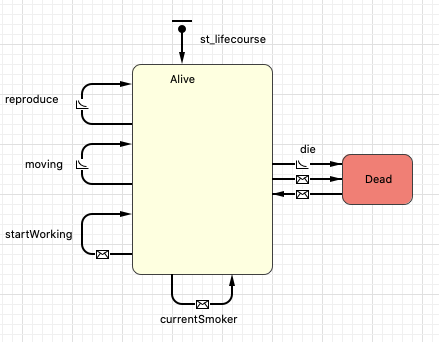
\includegraphics[scale=0.5]{plots/state_chart.png}
    % }
\end{figure}

\newpage
\begin{figure}[htp]
    \caption{\cite{chetty2014}'s rank-rank slope descriptives \newline CZ = Commuting zones}\vspace{5mm}
    \label{ch04:rank_slope_distribution}
     \centering
     \begin{subfigure}[b]{0.4\textwidth}
        %\caption{Number of kids}
         \centering
         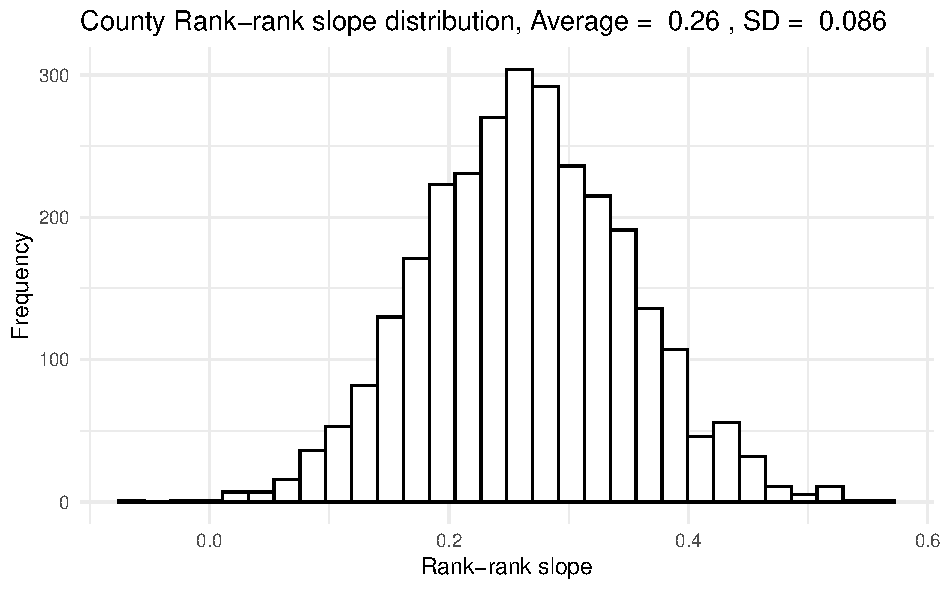
\includegraphics[width=\textwidth]{plots/rank-rank/cty_rrs_hist.pdf}
     \end{subfigure}
    %  \hfill
     \begin{subfigure}[b]{0.4\textwidth}
        %\caption{Age of death}
         \centering
         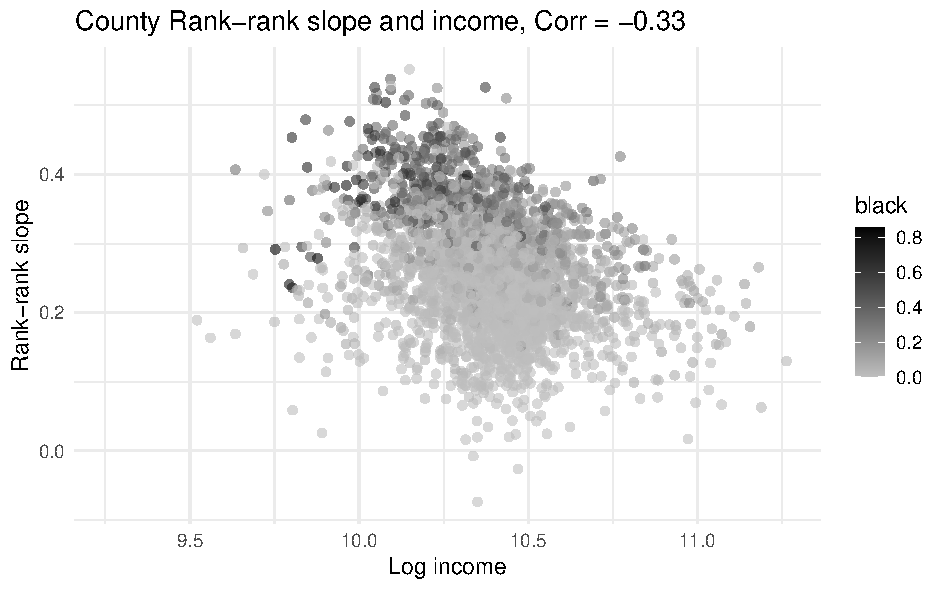
\includegraphics[width=\textwidth]{plots/rank-rank/cty_rrs_income.pdf}
     \end{subfigure}\vspace{5mm}

     \begin{subfigure}[b]{0.4\textwidth}
         %\caption{Life expectancy}
         \centering
         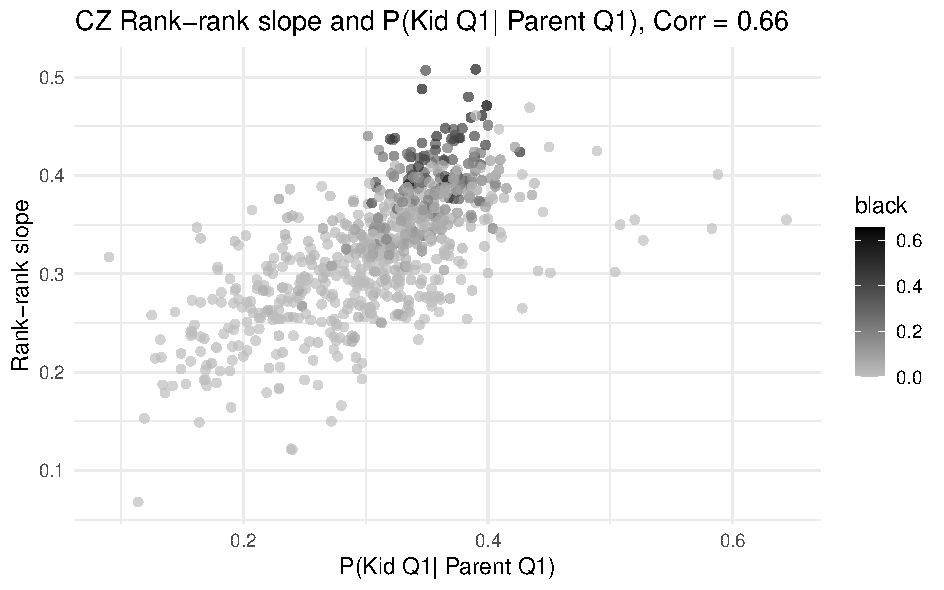
\includegraphics[width=\textwidth]{plots/rank-rank/cz_rrs_race_q1.pdf}
     \end{subfigure} %
     \begin{subfigure}[b]{0.4\textwidth}
        %\caption{Population size}
         \centering
         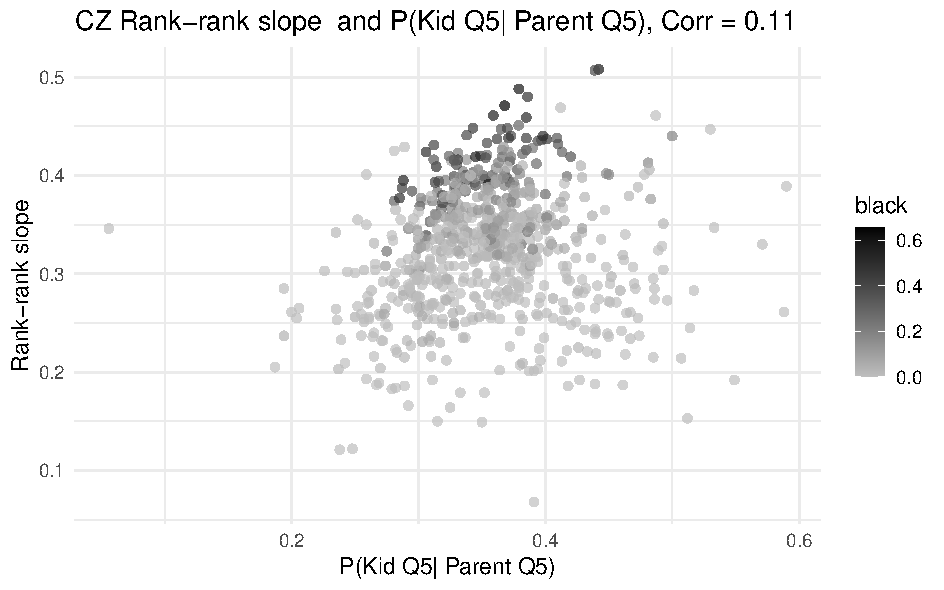
\includegraphics[width=\textwidth]{plots/rank-rank/cz_rrs_race_q5.pdf}
     \end{subfigure}
\end{figure}


\newpage
\begin{figure}[htp]
    \centering
    \caption{Agent's attributes and relationships}
    \label{ch04:agent_relationships}
        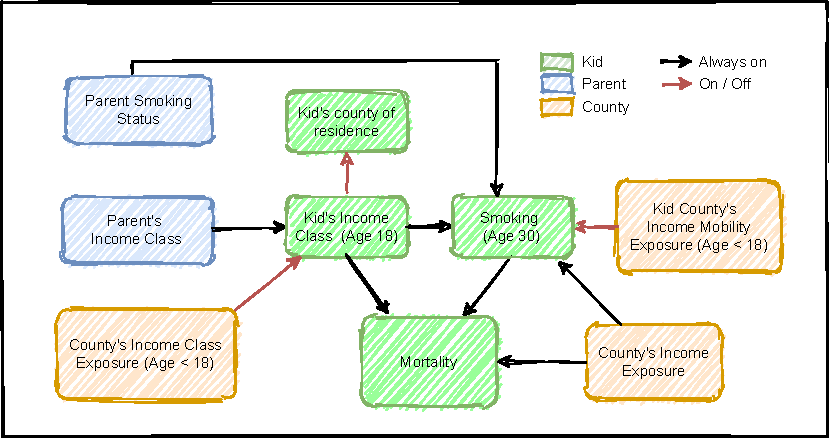
\includegraphics[scale=1.1]{plots/abm-mobility-simplified.pdf}
\end{figure}

\newpage
\begin{figure}[htp]
    \caption{Micro-simulated life expectancy (LE) differences for the\newline rank-rank slope effect on smoking} \label{ch04:microsimulation}\vspace{5mm}
     \centering
     \begin{subfigure}[b]{0.60\textwidth}
        % \caption{Number of kids}
         \centering
         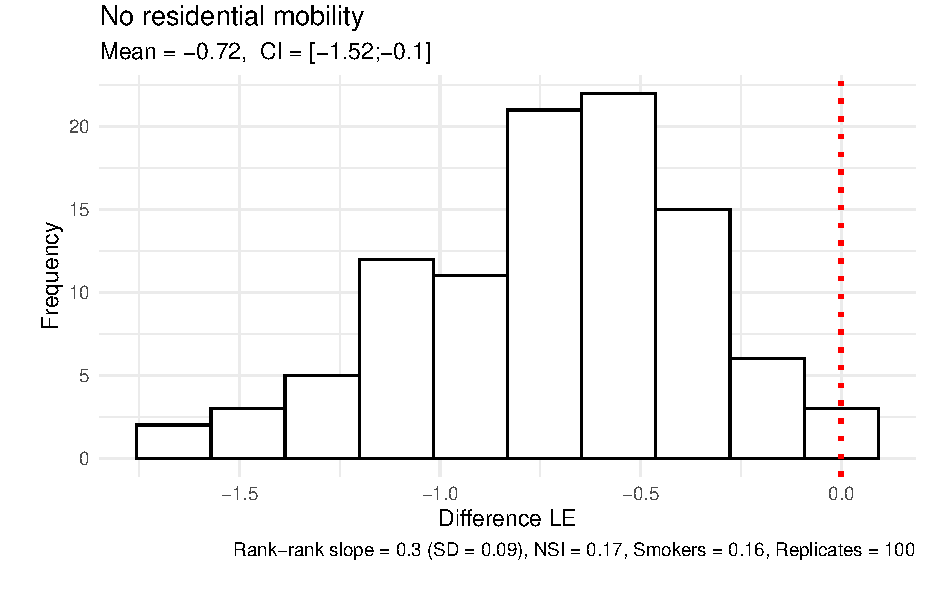
\includegraphics[width=\textwidth]{plots/microsimulation/microsimulation_1.pdf}
     \end{subfigure}\vspace{5mm}
     \begin{subfigure}[b]{0.60\textwidth}
        % \caption{Age of death}
         \centering
         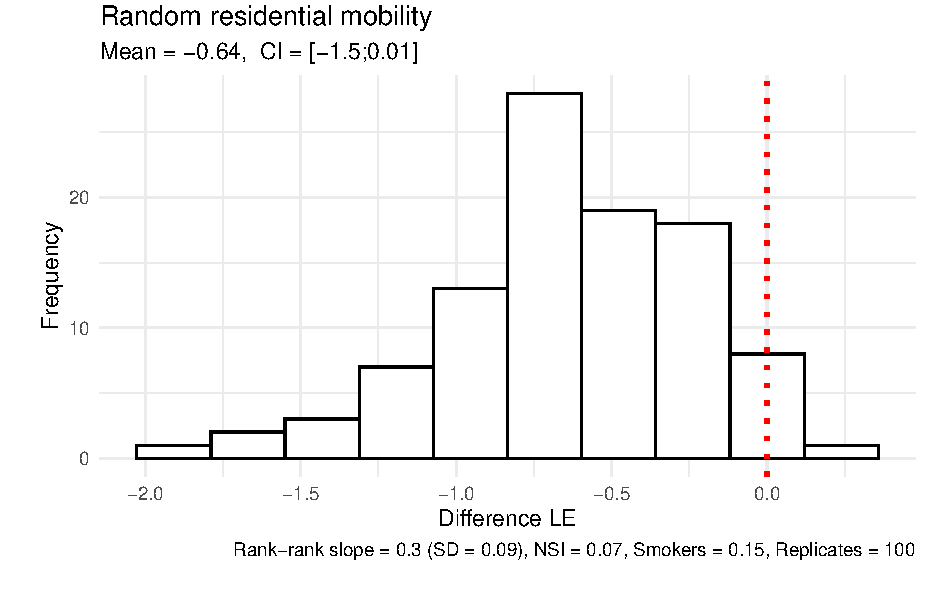
\includegraphics[width=\textwidth]{plots/microsimulation/microsimulation_2.pdf}
     \end{subfigure}\vspace{5mm}
     \begin{subfigure}[b]{0.60\textwidth}
         \centering
         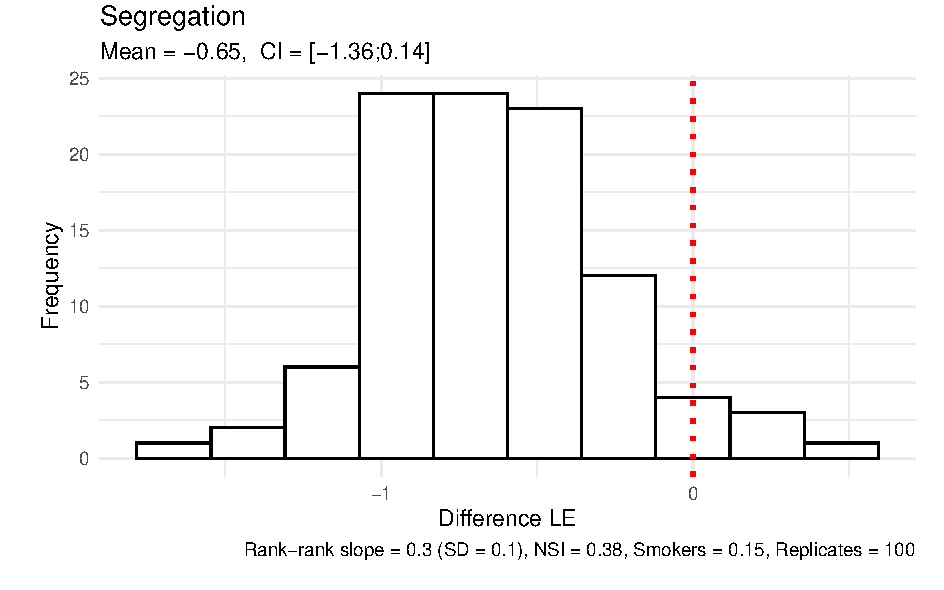
\includegraphics[width=\textwidth]{plots/microsimulation/microsimulation_3.pdf}
     \end{subfigure} %
\end{figure}


\newpage
\begin{figure}[htp]
    \caption{Micro-simulated life expectancy (LE) differences for the\newline rank-rank slope effect on smoking by income Q1 and Q5} \label{ch04:microsimulation_income}\vspace{5mm}
     \centering
     \begin{subfigure}[b]{0.50\textwidth}
         \centering
         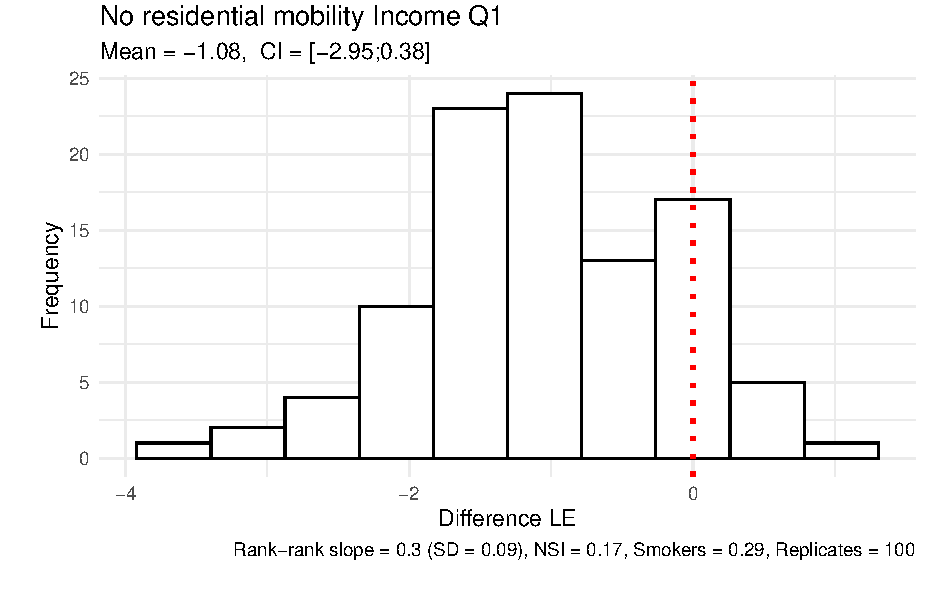
\includegraphics[width=\textwidth]{plots/microsimulation/microsimulation_1_1.pdf}
     \end{subfigure}%
     \begin{subfigure}[b]{0.50\textwidth}
         \centering
         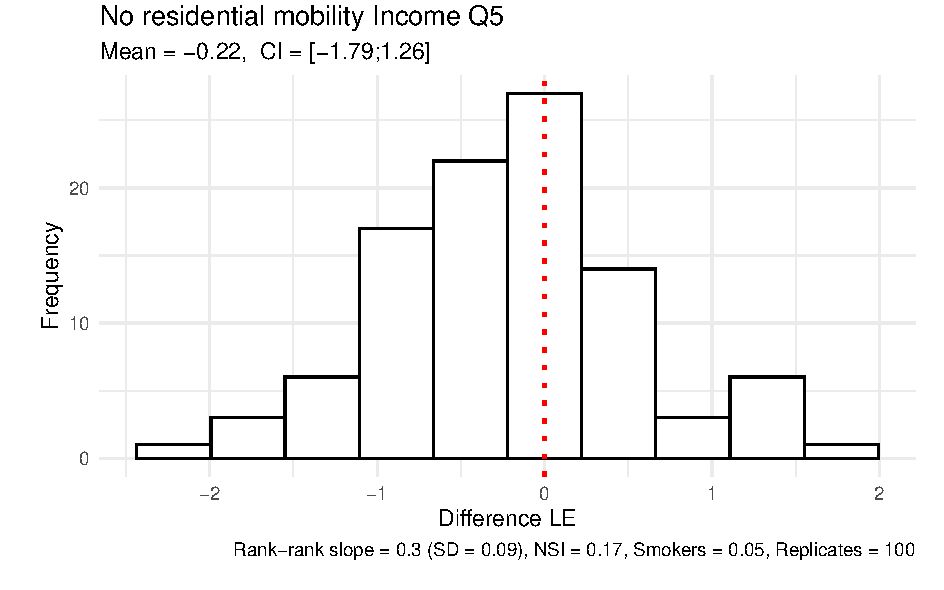
\includegraphics[width=\textwidth]{plots/microsimulation/microsimulation_1_5.pdf}
     \end{subfigure}\vspace{5mm}
     
     \begin{subfigure}[b]{0.50\textwidth}
         \centering
         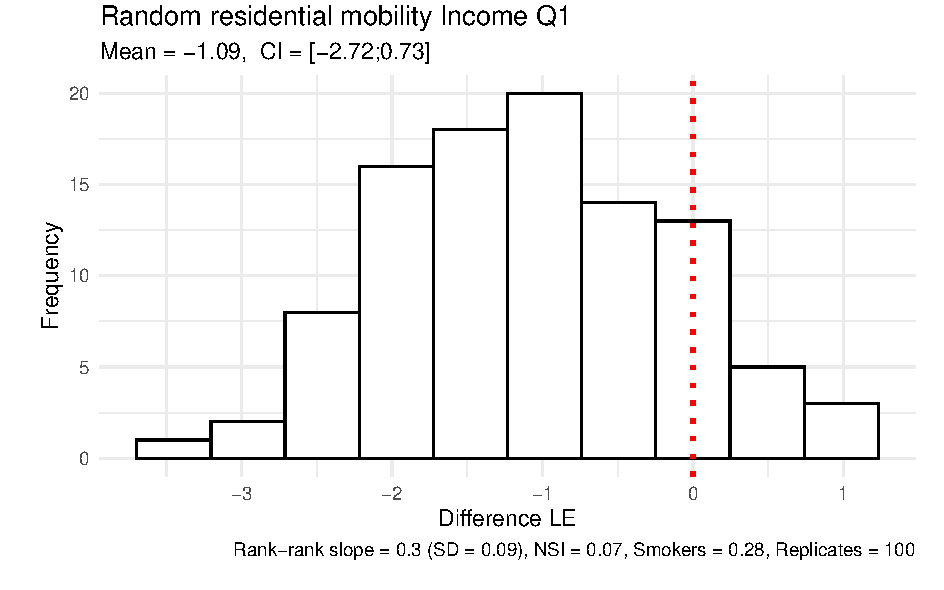
\includegraphics[width=\textwidth]{plots/microsimulation/microsimulation_2_1.pdf}
     \end{subfigure}%
     \begin{subfigure}[b]{0.50\textwidth}
         \centering
         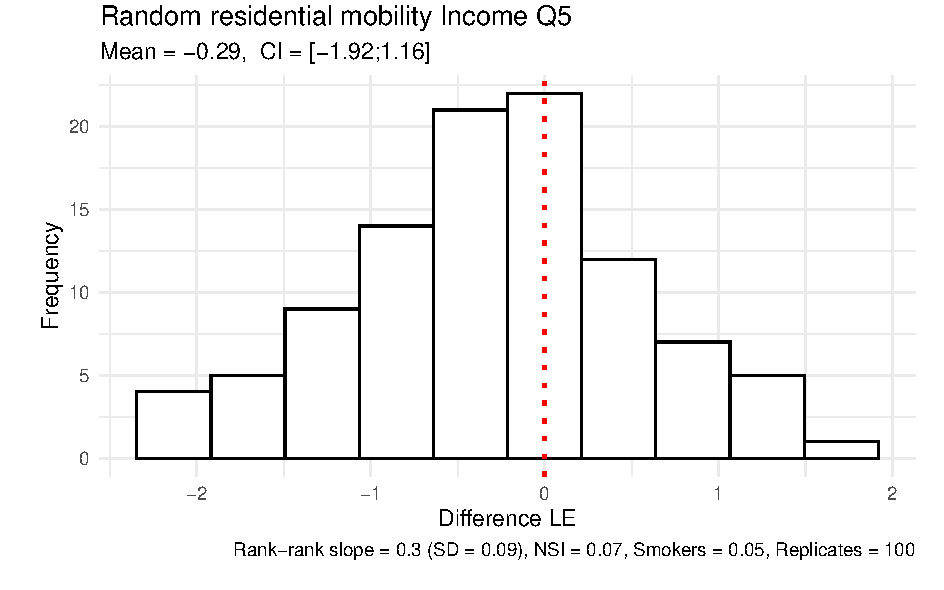
\includegraphics[width=\textwidth]{plots/microsimulation/microsimulation_2_5.pdf}
     \end{subfigure}\vspace{5mm}
     
     
    \begin{subfigure}[b]{0.50\textwidth}
         \centering
         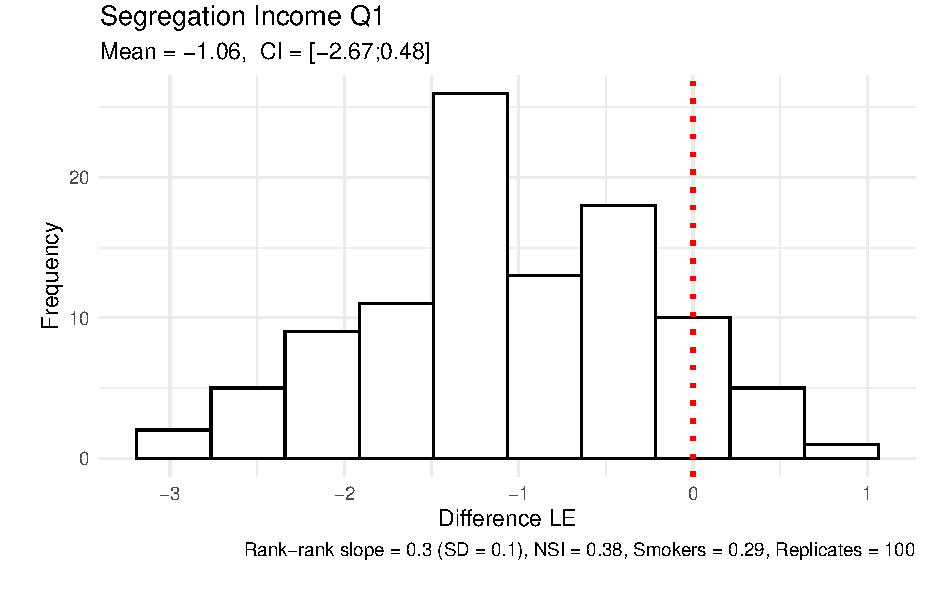
\includegraphics[width=\textwidth]{plots/microsimulation/microsimulation_3_1.pdf}
     \end{subfigure}%
     \begin{subfigure}[b]{0.50\textwidth}
         \centering
         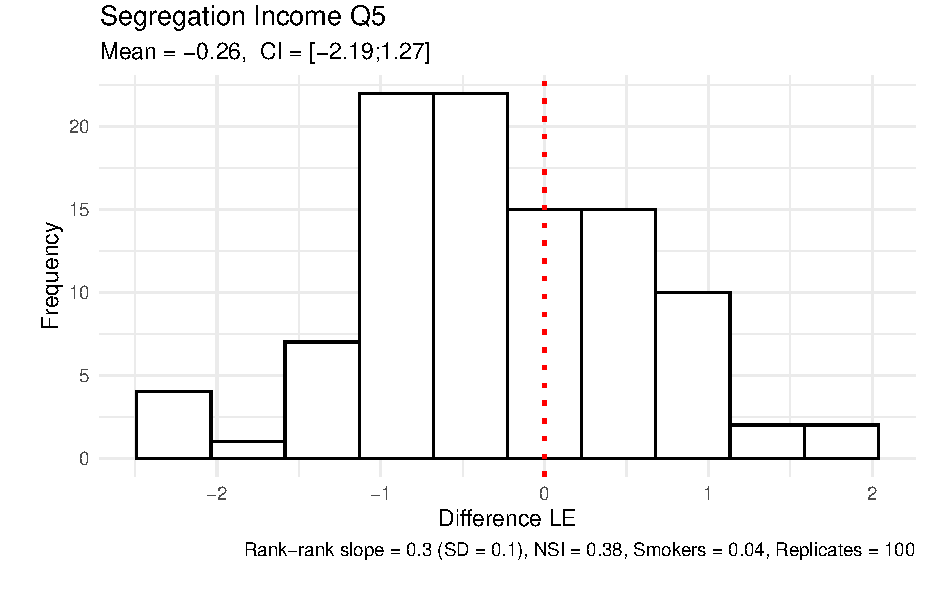
\includegraphics[width=\textwidth]{plots/microsimulation/microsimulation_3_5.pdf}
     \end{subfigure}
     
\end{figure}

\newpage
\begin{figure}[htp]
    \caption{Micro-simulated life expectancy (LE) differences for the\newline rank-rank slope effect on smoking using transition matrices as counterfactual} \label{ch04:microsimulation_transmob}\vspace{5mm}
     \centering
     \begin{subfigure}[b]{0.60\textwidth}
        % \caption{Number of kids}
         \centering
         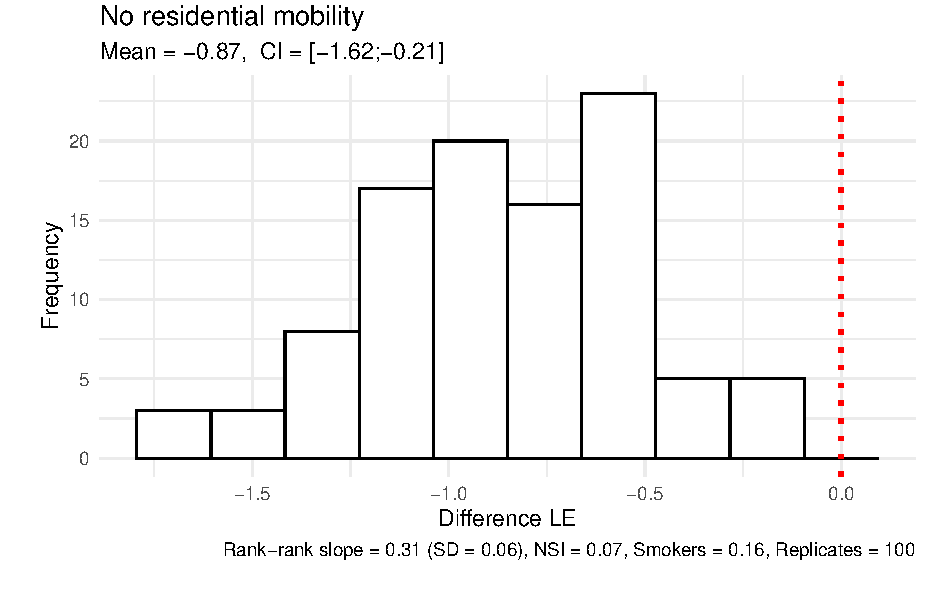
\includegraphics[width=\textwidth]{plots/microsimulation-transmob/microsimulation_transmob_1.pdf}
     \end{subfigure}\vspace{5mm}
     \begin{subfigure}[b]{0.60\textwidth}
        % \caption{Age of death}
         \centering
         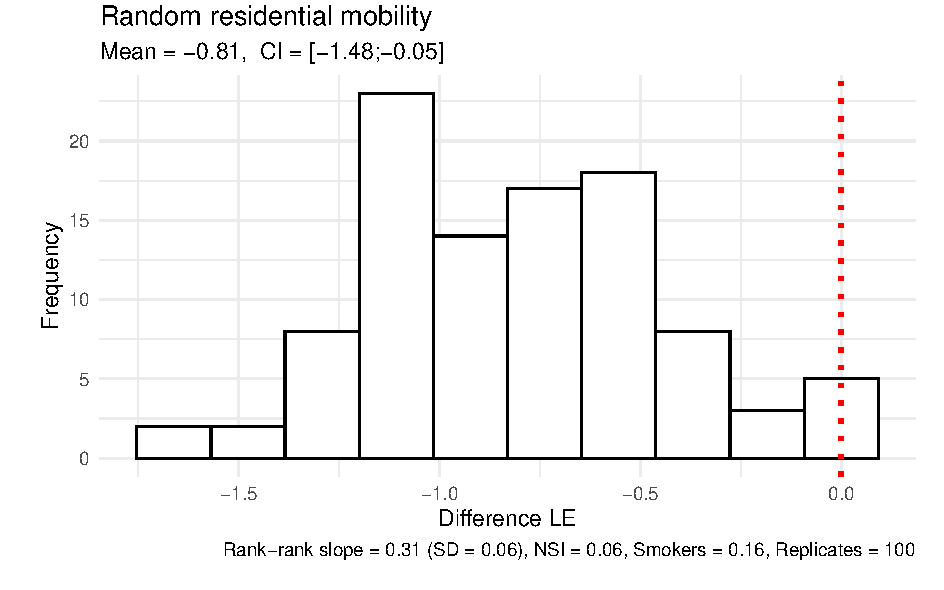
\includegraphics[width=\textwidth]{plots/microsimulation-transmob/microsimulation_transmob_2.pdf}
     \end{subfigure}\vspace{5mm}
     \begin{subfigure}[b]{0.60\textwidth}
         \centering
         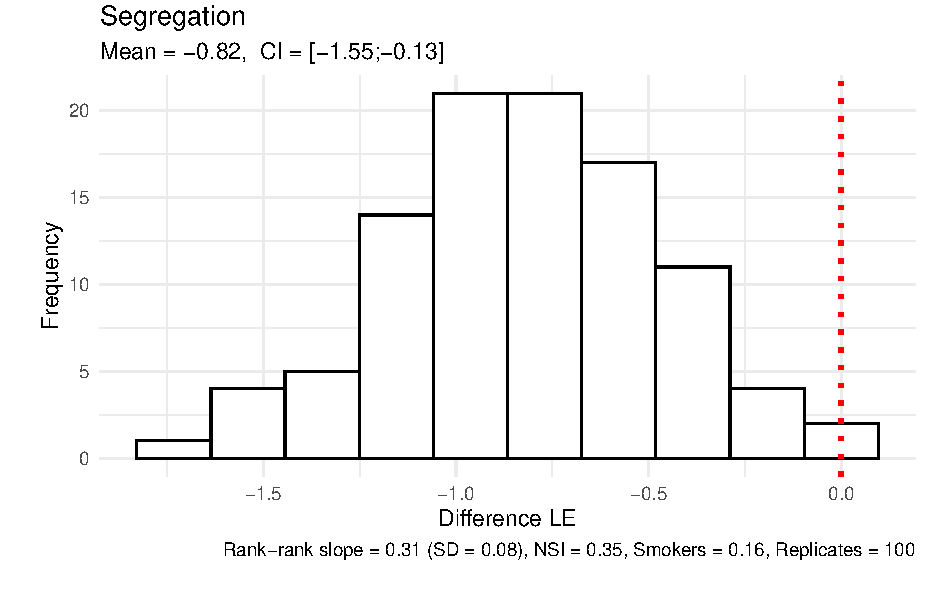
\includegraphics[width=\textwidth]{plots/microsimulation-transmob/microsimulation_transmob_3.pdf}
     \end{subfigure} %
\end{figure}


\onlyifstandalone{
\newpage
\setlength\bibitemsep{5pt}
\printbibliography[heading = subbibliography, title={References}]
\end{refsection}
}


% add supplement
\clearpage
\import{}{supplement}

%TC:endignore

\end{document}